\documentclass[a4paper, french, 12pt]{article}  % DŽclare la classe du document.
% Il existe 5 classes sous LaTeX : article, book, report, letter et slides 
% Les options de classe sont entre crochets et permettent de faire des choix d'ordre gŽnŽral :
% - dŽfinir la taille de base des caractres avec 10pt, 11pt, 12pt, les commandes d'agrandissement 
% ou de rŽduction de la tailles des caractres ( \small \large ) se feront alors par rapport ˆ cette base
% - dŽfinir la taille du papier:  a4paper,  a5paper, b5paper, executivepaper, legalpaper ou letterpaper
% Utiliser a4paper ds que la papier utilisŽ est de ce format c'est ˆ dire ... tout le temps ;-)
% - utiliser des options de mise en page : 
%       ->   landscape passe en mode paysage pour l'ensemble du doccument
%       ->   onecolumn  option par dŽfaut, le texte sera sur une seule colonne 
%       ->   twocolumn   pour un doccument sur deux colonnes, des rŽglages sont possibles (cf doc & net)
%       ->   oneside toutes les pages seront traitŽs identiquement, par dŽfaut avec la classe article
%       ->   twoside  mise en page diffŽrentes pour les pages pairs et impairs par dŽfaut avec book
%       ->   openright et openany  pour gŽrer le commencement des chapitres dans la classe book
%       ->   titlepage et notitlepage indique si une nouvelle page doit tre commencŽe aprs le titre du document.

% \usepackage permet de dŽclarer un module qui sera pris en compte dans la suite. 
% Les modules permettent d'Žtendre les fonctionnalitŽ de LaTeX

%%%%Caracteres reserves%%%%%%%%%%%
%Pour les obtenir on les fait précéder d'un \
% { s'obtient avec \{
% } s'obtient avec \}
% % s'obtient avec \%
% $ s'obtient avec \$
% & s'obtient avec \&
% # s'obtient avec \#
% _ s'obtient avec \_
% ^ s'obtient avec \^{}
% \ s'obtient avec \textbackslash{} car \\ est une commande
%Les caractères [ et ] ne sont pas réservés et s'obtiennent directement
%\[ et \] delimitent une environnement mathematique
%%%%%%%%%%%%%%%%%%%%%%%%%%%%%%%%%%%%%%%%%%%


%%%%%Polices%%%
%La police employee par defaut par Latex s'appelle Computer Modern

%%%Changement de style de police%%

%Police par defaut {\normalfont ...} c'est une bascule

%Trois familles 
%Romaine par defaut
%sans serif \textsf{..} ou {\sffamily ....}
%typewriter \texttt{..} ou {\ttfamily ....}

%Quatre formes
%droite par defaut
%italique \textit{..} ou {\itshape ....}
%penchee \textsl{..} ou {\slshape ....}
%petites capitales  \textsc{..} ou {\scshape ....}

%Deux series
%normale par defaut
%grasse \textbf{..} ou {\bfseries ....}


%%Taille%%
%Toutes les commandes suivantes sont des bascules a utiliser entre accolades
%{\tiny petit mot}
%Dans l'ordre croissant
%\tiny
%\scriptsize
%\footnotesize
%\small
%\normalsize
%\large
%\Large
%\LARGE
%\huge
%\Huge

%%%%%%%%%%%%%%%%%%%%%%%%%

%%%%%Justification%%%%%
%Alignement a droite
%\begin{flushright}
%{\raggedleft texte \par} ne pas oublier \par
%\leftline{texte}
%\filleft pour formater un titre 

%Alignement a gauche
%\begin{flushleft}
%{\raggedright texte \par} ne pas oublier \par
%\rightline{texte}
%\filright pour formater un titre 


%Centrage
%\begin{center}
%{\centering texte \par} ne pas oublier \par
%\centerline{texte}
%\filcenter pour formater un titre 
%%%%%%%%%%%%%%%%%%%%%%%%%%%%%%%%%%%%%%%%%%%

%%%%%%Espaces%%%%%%%%%%%%%%%%%%%%%


%%Espaces verticaux%%%
%\vskip 2cm  (argument eventuellement negatif), l'espace est ignore s'il coincide avec un saut de page
%\vspace*{2cm} (argument eventuellement negatif), l'espace n'est pas ignore s'il coincide avec un saut de page
%\vspace{2cm} est synonyme de \vskip 2cm 

%%Espaces horizontaux%%%%

%\hskip equivalent a \vskip
%\hspace{?} et \hspace*{?}
%Le cadratin est un espace horizontal egal a la taille de la police utilisee
%\thinspace espace d'un sixieme de cadratin
%\enskip pour un demi-cadratin
%\quad pour un cdratin
%\qquad pour deux cadratins

%%%%%%%%%%%%%%%%%%%%%%%%%%%%%%%%%%%%

%Le moteur eTeX est aujourd'hui utilisé par toutes les distributions (MikTeX, TeXlive) à la place de l'ancien TeX (en fait, c'est plutôt PDFTeX, le successeur de eTeX, qui est utilisé ; contrairement à ce que son nom indique, il peut produire du dvi). Le fait d'utiliser le moteur eTeX au lieu de TeX donne accès à des choses en plus (par exemple à \middle pour aller avec \left et \right, mais aussi à des commandes bien pratiques comme \numexpr, \dimexpr, \detokenize, etc. ainsi qu'à des ressources supplémentaires, comme plus de compteurs disponibles).

%Lorsqu'on utilise le moteur eTeX, certaines de ces fonctionnalités sont automatiquement accessibles (c'est le cas de \middle, \numexpr, etc.), mais pas d'autres (c'est le cas des compteurs supplémentaires). Pour activer ces fonctionnalités manquantes, on peut charger le package etex.sty. Ainsi, l'utilisation d'etex.sty est une solution courante au problème d'avoir trop de compteurs définis (c'est le cas si on charge ensemble trop de packages du type tikz, pstricks, xymatrix, ...)

\usepackage{etex}

%%%%%%%%%%%%Encodage du fichier source %%%%%%%%%%%
\usepackage[T1]{fontenc}
\usepackage[utf8]{inputenc}


%%%%%%%%%%%%%%%Francisation%%%%%%%%%%%%%%
\usepackage[french]{babel}
\frenchbsetup{StandardLists=true}
%%%%%%%%%%%%%%%%%%%%%%%%%%%%%%%%%%%%%%%%%

%%%%%%%%%%%%Mise en page, Reglages genrraux%%%%%%%

%\title{il n'existe pas de plus grand nombre premier}
%\author[Euclide \thanks{Merci Aristote}}
%\date{12 juin $-260$}  Par défaut Latex insère la date du jour
%puis écrire après \begin{document} la commande \maketitle


\usepackage[a4paper,headheight=35 pt, headsep=15pt,top=20 pt,hmargin=1 cm,bottom=20 pt,includeheadfoot]{geometry}
%\usepackage[a4paper,hmargin=1 cm,bottom=2cm,top=2cm,headheight=15pt]{geometry}      
%top est la marge supérieure entre le haut de body et le bord supérieur de la feuille
% \usepackage[left= 4cm,right = 3cm,top= 2cm, bottom=2cm]{geometry} pour le réglage des marges 
% \usepackage[top= 17mm,textheight=23cm,heightrounded,left=25mm,textwidth=16cm] {geometry} pour fixer la hauteur,  la largeur  du texte. heightrounded, autorise le package à arrondir la hauteur textheight à un nombre entier de lignes pour éviter des problèmes de remplissage vertical underfull vbox 


\usepackage{setspace}  % pour le réglage de l'interligne
%Bascule \doublespacing  ou environnement {doublespace}
%Bascule \onehalfspacing  ou environnement {onehalfspace}
%Bascule \singlespacing  ou environnement {singlespace}
% ou encore \renewcommand{\baselinestretch}{n} ou encore l'environnement spacing{n}

%%Package fullpage
%\usepackage[cm]{fullpage}
%where possible options for fullpage are
%in (default) sets the margins to one inch;
%cm sets the margins to 1.5 cm (one centimeter is really too
%little);
%plain (default) selects the plain page style, i.e., with no head-
%ers but only a footer;
%empty for neither headers nor footers;
%headings for both header and footers;
%myheadings also for both headers and footers.
%For the last 4 options, the corresponding \pagestyle declaration is exe-
%cuted, so that it is not necessary to give it again.


%%Pour la numerotation des bas de pages avec le compteur lastpage%%%
\usepackage{lastpage}

%%%%Pour afficher certaines pages au format paysage%%
\usepackage{lscape}
%\begin{landscape}

%%%Plusieurs colonnes
\usepackage{multicol}
%\begin{multicols}[titre]{nb colonnes}
\setlength{\columnseprule}{0.25pt}


%%%%%Références, Notes de bas de pages ou de marges%%%%%%%%%

%%Pour placer une note de bas de page : commande \footnote{}
%Pour placer une note dans la marge : \marginpar{}
%Pour plcaer une note dans un tableau : appel de note avec \footnotemark{} puis le texte après le tableau avec \footnotetext{texte}

%Etiquette  avec \label{nom} puis référence à l'étiquette (numéro de section le plus proche ) avec \ref{nom} ou à lap age avec \pageref{nom}
\usepackage{varioref}
%Introduit  les commandes \vref{} et \vpageref{} qui améloirent l'affichage ainsi que la commande \vpagerefrange{label1}{label2} pour faire référence à tout un bloc de pages entre deux étiquettes
\usepackage{nameref}


%%%%Présentation des titres de section%%%

%\usepackage[clearempty]{titlesec} problème avec PDFLatex ?

%Pour changer la police des titres de sectionnement, un exemple :
%\titleformat*{\section}{\sffamily}

%Pour modifier la police mais aussi la présentation :
%\titleformat{commande}[shape]{format}{label}{sep}{before}{after}
% commande est la commande de sectionnement comme \section
%shape peut etre hang (défaut),frame (encadre), display( paragraphe séparé), block (paragraphe), runin (dans le texte, wrap (comme wrapfigure), leftmargin ou rightmargin
%format est le formatage du titre complet (numéros inclus)éventuellemnt précédé de commandes à inclure avant le titre
% Ces commandes peuvent etre \titleline[r,c ou l]{texte} ou \titlerule[epaisseur] ou \titlerule*[epaisseur]{texte}
%label est la présentation du numero
%sep est l'espace entre le numero et le titre
%before est le code à exécuter avant le titre de section (numero exclu)
%after est le code à exécuter après (vide en général)

%Pour gérer l'espacement
%\titlespacing{commande}{left}{beforesep}{aftersep}[right]
%left est la marge à gauche, beforesep l'espace vertical avant etc ..


%Exemple de présentation de titre encadé :
%\titleformat{\section}[frame]{\titleline[r]{\rule{2in }{2pt}} \normalfont}{\filright\small\ SECTION \thesection\hfill}{7pt}{\LARGE \bfseries\filcenter}{}
%\section{un titre de section encadre}


%%%%%%%%%%%%%%%%%%%%%%%%%%%%%%%%%%%%%%%%%%%% 

%%%%%%%Réglages de la table des matières%%%%
\usepackage{tocvsec2}
%Définir la progondeur : \setcounter{tocdepth}{1}  :
%1 correspond aux chapitres; 2 aux sections etc ...
%Rédéfinir le nom par défaut  :
%\renewcommand{\contentsname}{Liste des chapitres}
%Modifier une entrée :
%\Chapter[titre court]{titre long}
%Ajouter une entrée :
%\addcontentsline{toc}{section}{Nom de la section qu'on veut ajouter}
%Pour exclure une entrée 
%Utiliser une commande étoilée comme \section*
%Pour ajouter  ce qu'on veut dans la table des matières comme des indications de mise n page :
%\addtocontents{toc}{\protect \pagebreak}


%%%%%%%%%%%% Packages pour le texte %%%%%%%%%%%%
\usepackage{lmodern}       %Joli fonte

\usepackage{pifont,fourier}
\usepackage[normalem]{ulem}
%\uline{} pour  un soulignement simple
%Commmandes \uuline{} pour un soulignement double
%\uwave{} pour un soulignement  avec des vagues
% \sout{} pour barrer et \xout{} pour hachurer
\usepackage{cancel} %Commande \cancel{} pour barrer en oblique
%\usepackage{soul}    %souligner
%\usepackage{lettrine} %Pour commencer un paragraphe avec une lettrine
%Package incompatible avec tabvar.tex
%\lettrine{S}{i vous souhaitez}
%\renewcommand{\LettrineFontHook}{\itshape}
%\renewcommand{\LettrineTextFont}{\sffamily}

%%%Pour des jolis boites%%%
\usepackage{fancybox}  
%Commandes \box{} \ovalbox{} \shadowbox{}
%\cornersize{}2 réglage de l'arrondi
% Dimension à régler avec \setlength{}  : \fboxsep \fboxrule  

%%% Pour faire tourner le texte %%%
\usepackage{rotating}  %\begin{turn}{-60} tourné \end{turn} pour tourner un paragraphe
						%pour tourner un texte, commande \rotatebox[origin=c]{angle}{texte}
						
%%Divers%%%%
\usepackage{eurosym}  %pour le symbole de l'euro

\usepackage{url} %pour la gestion des adresses web avec la commande \url{}

%%%%%%%%%%%

%%%%%%%%%%%%%%%Ecriture d'algorithmes Insertion de code source %%%%%%%%%%%

%%%%%Package verbatim%%%%

\usepackage{verbatim} 
%LE package verbatim améliore la présentation des verbatim
% Il  fournit un environnement {comment} pour insérerer des commentaires
%dans le fichier source sans faire précéder toutes les lignes de %

\usepackage{alltt, moreverb} 
%L'environnement verbatimboxed permet d'encadrer un texte en verbatim
% De plus les caractères spéciaux \ et { ne sont pas désactivés (mais #, $ et % le sont)
% et on peut saisir des formules mathématiques avec \( .. \) ou \[ ... \]

%%Pour améliorer envore la présentation des verbatim%%%%
\usepackage{fancyvrb}


%%Couleur
\usepackage[table]{xcolor}
% options : rgb,cmyk,gray,hsb,html pour transformer automatiquement toutes les couleurs du docuement dans le mode choisi
%\definecolor{mauve}{rgb}{0.7,0,0.43}
%\color{couleur} bascule
%\textcolor{couleur}{texte}
%\pagecolor{couleur}
%\colorbox{couleur}
%\fcolorbox{couleur}




%%%%%%%%%%%%%%%%%%¨Puce, Listess%%%%%%%%%%%%%%
\usepackage{enumerate}
\usepackage{enumitem}
%Pour changer la puce de liste dans tout le document :
%AtBeginDocument{\renewcommand{\labelitemi}{\textbullet}}
%%%%%%%%Réglages spécifiques au document%%%%%%%%%

%\setenumerate[1]{label=\textbf{Q\arabic*)}}


%%%%%%%%%%%%Graphiques et Dessins%%%%%%%%%%%%%%

\usepackage{graphicx}		
%\rotatebox[origin=x0x1]{angle}{texte} avec xox1 parmi t (top) l (left) r (right) B (ligne de base) et b (bottomm)
%\resizebox{largeur}{hauteur}{texte} pour faire rentrer u nelement encombrant dans une boite					


\usepackage{epic,eepic}   %Capacités graphiques étendues
%\begin{picture}(0,0) permet d'insérer n'importe quoi, n'importe où sans prendre de place (utilie pour annoter une figure en eps)
%Une autre technique est \makebox[0cm][alignement]{texte}
%Exemple:
%\includegraphics[scale=1]{singe.eps}
%\begin{picture}(0,0)
%\put(-27,10){$\sqrt[3]{8}$}
%\end{picture}



%%%%%%%%%%PSTricks%%%%%%%%%%%%

\usepackage{pstricks,pst-plot,pst-text,pst-tree,pst-eps,pst-fill,pst-node,pst-math,pstricks-add,pst-xkey,pst-eucl}


%%%%%%%Tikz%%%%%%%%%%%%%%%
\usepackage{pgf,tikz,tkz-tab}
% Pour les tableaux de signes ou de variations avec tkz-tab voir https://zestedesavoir.com/tutoriels/439/des-tableaux-de-variations-et-de-signes-avec-latex/#1-13389_tikz-un-package-qui-en-a-dans-le-ventre
\usetikzlibrary{arrows}
\usetikzlibrary{shapes.geometric}
\usetikzlibrary{petri}
\usetikzlibrary{decorations}
\usetikzlibrary{arrows}
\usetikzlibrary{math}
 %Variables must be declared in a tikzmath environment but
       % can be used outside
%       \tikzmath{int \n; \n = 508; \x1 = 1; \y1 =1; 
%                   %computations are also possible
%                    \x2 = \x1 + 1; \y2 =\y1 +3; } 



%%%%%%%%%%%%%%%%%%%%%%%%%%%%%%%%%%%%%%%%
%%%%%%%%%%%Commandes Tikz Perso%%%%%%%%%%%%%%%

% Définition des nouvelles options xmin, xmax, ymin, ymax
% Valeurs par défaut : -3, 3, -3, 3
\tikzset{
xmin/.store in=\xmin, xmin/.default=-3, xmin=-3,
xmax/.store in=\xmax, xmax/.default=3, xmax=3,
ymin/.store in=\ymin, ymin/.default=-3, ymin=-3,
ymax/.store in=\ymax, ymax/.default=3, ymax=3,
}
% Commande qui trace la grille entre (xmin,ymin) et (xmax,ymax)
\newcommand {\grille}[2]
{\draw[help lines,black, thick] (\xmin,\ymin) grid[xstep=#1, ystep=#2] (\xmax,\ymax);}
% Commande \axes
\newcommand {\axes} {
\draw[->,very thick] (\xmin,0) -- (\xmax,0);
\draw[->,very thick] (0,\ymin) -- (0,\ymax);
\draw (0.95*\xmax, 0) node[above] {$x$};
\draw (0, 0.95*\ymax) node[left] {$y$};
}
% Commande qui limite l?affichage à (xmin,ymin) et (xmax,ymax)
\newcommand {\fenetre}
{\clip (\xmin,\ymin) rectangle (\xmax,\ymax);}

%Exemple d'utilisation

%\begin{center}
%\begin{tikzpicture} [xmin=-2,xmax=2,ymin=0,ymax=5]
%\grille{1} \axes \fenetre
%\draw plot[smooth] (\x,\x^2);
%\end{tikzpicture}
%\end{center}

%style pour la perspective cavalière française
%voir Tikz pour l'impatient page 68
\tikzset{math3d/.style=
{x= {(-0.353cm,-0.353cm)}, z={(0cm,1cm)},y={(1cm,0cm)}}}

%%%%%%%Symbole pour code calculatrice%%%%%%

%Flèche remplie pour défilement de menu

\newcommand{\flechefillright}{
\begin{tikzpicture}[scale=0.15] \fill (0,0)--(2,1)--(0,2)--cycle;
\end{tikzpicture}}

%%%%%%%%%%%%%Symboles pour calculatrice Casio%%%%
\newcommand{\execasio}{\Pisymbol{psy}{191}} %Retour chariot
\newcommand{\dispcasio}{\begin{pspicture}(.1,.1)\pspolygon*(.1,0)(.1,.1)\end{pspicture}} %Triangle « Disp »
\newcommand{\dispcasiotikz}{\begin{tikzpicture}[scale=0.2]
\fill (0,0) -- (1,0) -- (1,1) -- cycle;
\end{tikzpicture}} %Triangle « Disp »
%

%Fleche entre deux lignes, d'apres 'un bon petit' : http://forum.mathematex.net/latex-f6/fleches-entre-deux-lignes-pour-resolution-d-equation-t10283.html#p99817
\newcommand\addnode[1]{\Rnode{#1}{}}
\newcommand\linknode[3]{\ncbar[angleA=0,angleB=0,nodesep=1ex,arm=10ex,offset=-2pt]{->}{#1}{#2}\Aput{\vphantom{x}#3}}

%%%%%%%%%%%%%%%%%%%%%%%%%%%%%%%%%%%%%%%%
%%%%%%%%%%%Fin Commandes Tikz%%%%%%%%%%%%%%%


%%%%%%%%%%%%Specifiques%%%%%%%%%%%
\usepackage{wrapfig}
%pour insérer une figure à droite ou à gauche d'un texte
%\begin{wrapfigure}[nb lignes]{placement l,r,c,i(inside),o(outside)}[overhang]{width}
%ce package fonctionne mal à proximité des listes
%%%%%%%%%%%%%%%%%%%%%%%%%%%%%%%%%%%%%

%%%%%Environnements et symboles spéciaux pour faire joli%%%%%%

%%%Pour des environnements + jolis avec insertion de logo%%%%
\usepackage{xkeyval}  %indispensable pour bclogo
\usepackage[tikz]{bclogo}

\usepackage{framed}  %Le package « framed» Crée 3 nouveaux environnements, qui se comportent comme des minipage de largeur \linewidth, mais permettant en plus de se casser entre plusieurs pages.     * framed : avec un cadre autour;     * shaded : avec un fonc coloré (il faut définir la couleur shadecolor);     * leftbar : avec une barre le long du côté gauche.

%%%%%%%%%%%%%%%%%%%%%%%%%%%%%%%%%%%


%%%%%%Environnements et symbomles mathématiques%%%%

%%%Tableaux de variations %%%%%%%%%%

\usepackage{variations}

%%%%%%%%%%%AmsMaths%%%%%%
\usepackage{mathtools}        %Commandes essentielles, extension d'amsmath
\usepackage{amsfonts,amssymb}  %Principaux symboles
\usepackage{mathrsfs} %Polices calligraphiques
\usepackage{stmaryrd} %Pour les intervalles d'entiers avec \llbracket et \rrbracket
\usepackage[autolanguage, np]{numprint}
%%%%%%%%%%%%Là encore il y a de grosses différences entre le monde anglo-saxon et les francophones.Le séparateur des décimales est un point en anglais et une virgule en français. Leséparateur des milliers est une virgule en anglais et une espace insécable en français. Ilest préférable d’utiliser le package numprint (\usepackage{numprint}) qui associé àfrenchb produira la bonne typographie.
%123456789 = 123456789 \numprint{123456789} = 123 456 789  \numprint{3,1415926535897932384626} = 3,141 592 653 589 793 238 462 6  \numprint{12.34} = 12,34  En plus tu peux préciser les unités de cette façon : \numprint[kg]{12.34} = 12,34 kg ou encore \numprint[\degres C]{22} = 22°C Si tu veux utiliser le raccourci \np{} au lieu de \numprint{}, il te faut charger le package de cette façon : \usepackage[np]{numprint}
\usepackage[thmmarks,amsmath]{ntheorem}
%Pour définir un nouveau théorème :
%\newtheorem{conj}{Conjecture}[chapter] environnement con d'en tete Conjecture avec numérotation au sein d'un chapitre
%Pour rédéfinir le style d'un théorème, placer les commandes avant \newtheorem et entourer le tout d'accolades
%\theoremstyle{style} : :
% plain est le style par défaut
% break insère un saut de ligne après le titre du théorème
%margin et marginbreak sont les équivalents avec numéro dans la marge
%\theorembodyfont{\normalfont \sffamily} police du corps du théorème
%\theoremheaderfont{\scshape} police de l'en-tete (définie 1 fois pour tous les théorèmes)
%\theoremsymbol{ } symbole ajouté à la fin du théorème
%\theoremseparator{--} élément situé entre le numéro et le corps du theoreme
%\theoremprework{\rule{\linewidth}{0.4pt}} élément précédant chaque théoreme
%\theorempostwork{\dingline{71}} élément suivant chaque théoreme
%\theoremnumbering{Roman} style de numérotation
\usepackage{bbm, dsfont}   %Fonction indicatrice
\usepackage{esint,esvect}  %Flèches supplémentaires.
\usepackage{lcg}  %%%%%%%générer des nombres pseudo aléatoires%%%%


%%%%%%%%%%%Tableaux%%%%%%%%%%%
\usepackage{array}
%\usepackage{multirow} %problème redéfinit la commande \multirow{nligne}*{texte}
\usepackage{tabularx}        % Largeur totale donnée          
\usepackage{longtable}       %Sur plusieurs pages
%\usepackage{diagbox}  %Successeur de slashbox, voir Latex pour l'impatient p. 73, charge pict2e qui redefinit \arc
\usepackage{alterqcm} 
%%%Une commande de David Robert%%%%%%%
%\newcommand{\delair}[1]{\ensuremath\displaystyle\psframebox[framesep=0.15em,linestyle=none]{ \displaystyle#1}}
\newcommand{\delair}[1]{\setlength{\fboxrule}{0mm} \fbox{#1}}
%%%%%%%%%%%%%%%%%%%%%%%%%%%%%%%%%%%%%%




%%%%%%%%%%%%%%Programmation en Latex, Création de nouvelles Commandes%%%%%%%%%%%%%
\usepackage{xspace} %pour la gestion fine des espaces avec la commande \xspace
\usepackage{calc} %   pour faire des calculs avec les longueurs par exemple%%
%Commande \real{0.72} pour le reel 0,72
%\ratio{3}{4} pour le reel 0,75

\usepackage{ifthen}
%Syntaxe d'un test conditionnel : \ifthenelse{condition}{action si realisee}{action sinon}
%Commandes de test :
%\isodd{entier}
%\equal{chaine 1}{chaine 2}
%\lengthtest{comparaison entre deux longueurs} retourne un booleen
%\or, \and, \not \( et \) permettent de combiner des tests avec parenthesages
%
\usepackage{multido}  % package pour utiliser de boucles iteratives

%%%%Boucle Pour%%%

% Sa syntaxe est la suivante : 
% \multido{variables}{nbiteration}{code}
% Le code sera ainsi repete nbiteration fois. Les declarations de variables sont separees par des virgules. Un declaration prend la forme :
%    variable = valeurinitiale + increment  Exemple :
% \multido{\i=0+1}{21}{instruction a repeter } 
%Les variables d'initialisation commencent par i s'il s'agit d'entier, par r s'il s'agit de reels et par d sis ce sont des longueurs
%Exemple de calcul des multiples de pi et d'affichage un par ligne :
%\newcommand{\multipledepi}[1]{\multido{\ia=2+1,\rpi=6.28318530+3.14159265}{#1}{$\ia\pi\approx\rpi$\endgraf}
%Noter que la commande \endgraf synonyme de \par est bien prtique dans les commandes ou \par est interdite

%%%%%Boucle Tant Que%%
%Syntaxe : \whiledo{test}{instruction}
%Exemple d'affichage de lignes pointillees pour laisser la place dans un enonce de controle avec \reponses{7} par exmeple (on peut aussi utilsier \multido dans ce cas)
%\newcounter{nombreentier}
%\newcommand{\reponses}[1]{\setcounter{nombreentier}{0}\whiledo{\value{nombreentier}<#1}{\noindent \dotfill \par \stepcounter{nombreentier}}}



%%%%%%%%%%%%%%%%%%%%%%%%%%%%%%%%%%%%%%%%%%%%%%


%%%%%%%%%%%%%%%%%%%%%%%Longueurs%%%%%%%%%%%%%%%%%%%%%%%%%%

%Attention a la syntaxe :
% Si on a une longueur appelle \longueur :
%\rule{0.72\longueur}{1mm} pas de *
%mais \rule{\real{0.72}*\widthof{exemple}}{1mm}

%unites de longueur : pt, mm, cm ect
%unites qui dependent de la police utilisee : 1 em correspond à l longueur d'un m et 1 ex à la hauteur d'un x
%\setlength{\nom}{valeur}
%\addtolength{\nom}{valeur}
%\settowidth{\nom} \settoheigth{\nom}

%%%%%%Boites avec longueurs caracterisitiques%%%
%\fbox \makebox \framebox utlisent stockent dans \height, \width, \depth, \totalheight les dimensions de l'argument de la commande
%Exemple : \framebox[\width+17mm][positionnement]{un texte encadre}
%DE fçon plus generale on peut acceder aux dimensions d'un objet avec :
%\widthof{texte} \depthof{texte} \heightof{texte}
%Exempel : \rule{\widthof{un exemple}}{1mm}


%%%%%%%%%%%%%%Compteurs%%%%%%
%Un compteur comme celui qui numerote les sections  represente 3 elements distincts  :
%D'abord son nom section
%Ensuiet sa valeur en tant qu'entier : \value{section} (qui vaut 6 dans l'exemple mais qui ne s'affiche pas directment, elle sert d'argument pour d'autres commandes)
%Enfin son apparence \thesection qui affiche par exemple 11.6  pour section 6 du chapitre 11

%Definition d'un nouveau compteur : \newcounter{moncompteur}
%\newcounter{nom}[old] indique que le compteur nom est remis à 0 lorsque le compteur old est a 0
%initialisation : \setcounter{moncompteur}{0}
%ajout d'une valeur : \addtocounter{moncompteur}{valeur} pour ancienne valeur + valeur
%incrementation de 1 : \refstepcounter{moncompteur}
%Pour mieux gerer la remise à 0 d'un compteur en foinction d'un autre compteur :
%\numberwithin{moncompteur}{autrecompteur}

%%%%Redefinition d'un compteur deja existant :
%D'abord on choisit le type de numerotation (\roman \Roman \Arabic \arabic \alpha \Alpha)
\renewcommand{\theenumi}{\textbf{\arabic{enumi}}}
%Puis on choisit l'apparence de l'etiquette
\renewcommand{\labelenumi}{\textbf{\theenumi.}}
\renewcommand{\theenumii}{\textbf{\alph{enumii}}}
\renewcommand{\labelenumii}{\textbf{\theenumii.}}



%%%%%Package à appeler après Babel%%%%%%%%%%%%

%%%%%%%%Flottants%%%%%%%%%%%%%%%%%%%%%%%%
%packages qui doivent etre chargés après le package babel
%car ils utilsient le package caption
\usepackage{float,afterpage}
%Deux types de flottants par défaut : figure et table
%\begin{figure}[préférences de placement dans l'orde de gauche à droite: t,,b,h,p,h!,H]
%\caption[texte court pour la liste]{légende}
%Liste des flottants ; \listoffigures ou \listoftables ou  \listeof{flottant}{titre}
%Placements par défaut pour tout le document: \floatplacement{figure}{t}
%Légende avec \caption{Légende} suivie de \label{Etiquette}
%Quand un flottant passe en mode p aucun autre flottant ne peut etre inséré
%tant qu'une page entire de flottants n'a pas été composée
%Pour vider le stocke de flottants on utilise la commande \clearpage
%\clearpage force u nsaut de page et réserve la page suivante aux flottants
% Pour finir la page en cours, utiliser \afterpage{\clearpage} 

%Défintion de nouveaux flottants
%\newfloat{nom}{positionnement}{extension du fichier de liste}[compteur d'appui]
%\newfloat{ex}{hb}{loex}[chapter]
%\floatname{ex}{\textit{Exemple}} nom dans la légende du flottant
%\floatstyle{boxed}
%\listof{ex}{Liste des exemples de code}

\usepackage[section]{placeins}
%pour que les flottants soient bien inclus dans la section à laquelle ils appartiennent

\usepackage{subfig}
%sous-flottants
%\subfloat[légende]{sous-flottant}
%Pour faire apparaitre les sous-flottants dans la liste des flottants :
%\setcounter{lofdepth}{2}

\usepackage{caption}  %Pour les légendes
%voir Latex pour l'impatient page 94 (pour la commande \captioof{type de flottant}[texte court] {texte}
%voir Latex pour l'impatient page 94 pour le paramétrage  des options de légendes

%%%%%%%%%%%%%%%%%%%Présentation de codes sources%%%%%%%%%%%%%%%%%
\usepackage{listings}
%On utilise l?environnement lstlisting pour insérer
%un code source.
%En plus de l?environnement lstlisting, on peut également utiliser la
%commande \lstinline qui fonctionne comme la commande \verb, en ce
%sens qu?on peut utiliser n?importe quel caractère comme délimiteur. Enfin,
%la commande \lstinputlisting permet de charger un code source depuis
%un fichier externe.
%Il y a deux manières de préciser des options : soit via l?option de l?envi-
%ronnement ou de la commande, soit en utilisant la commande \lstset
%qui permet de définir des options de manière globale.

\lstset{ %
  language=Python,                % the language of the code
  basicstyle=\ttfamily,           % the size of the fonts that are used for the code
  %numbers=left,                   % where to put the line-numbers
  numberstyle=\tiny,  % the style that is used for the line-numbers
  %stepnumber=2,                   % the step between two line-numbers. If it's 1, each line 
                                  % will be numbered
  %numbersep=5pt,                  % how far the line-numbers are from the code
  backgroundcolor=\color{white},      % choose the background color. You must add \usepackage{color}
  showspaces=false,               % show spaces adding particular underscores
  showstringspaces=false,         % underline spaces within strings
  showtabs=false,                 % show tabs within strings adding particular underscores
  frame=single,                   % adds a frame around the code
  rulecolor=\color{black},        % if not set, the frame-color may be changed on line-breaks within not-black text (e.g. comments (green here))
  tabsize=4,                      % sets default tabsize to 2 spaces
  captionpos=b,                   % sets the caption-position to bottom
  breaklines=true,                % sets automatic line breaking
  breakatwhitespace=false,        % sets if automatic breaks should only happen at whitespace
  %title=\lstname,                   % show the filename of files included with \lstinputlisting;
                                  % also try caption instead of title
  breakindent=1cm,
  keywordstyle=\color{blue},          % keyword style
  commentstyle=\color{red},       % comment style
  %stringstyle=\ttfamily\color{green},         % string literal style
  escapeinside={\%*}{*)},            % if you want to add LaTeX within your code
  morekeywords={*,...},              % if you want to add more keywords to the set
  deletekeywords={...}              % if you want to delete keywords from the given language
  upquote=true,columns=flexible,
xleftmargin=1cm,xrightmargin=1cm,
 inputencoding=utf8,			%Les lignes qui suivent sont pour le codage utf8
  extendedchars=true,
  literate=%
            {é}{{\'{e}}}1
            {è}{{\`{e}}}1
            {ê}{{\^{e}}}1
            {ë}{{\¨{e}}}1
            {û}{{\^{u}}}1
            {ù}{{\`{u}}}1
            {â}{{\^{a}}}1
            {à}{{\`{a} }}1
            {î}{{\^{i}}}1
            {ô}{{\^{o}}}1
            {ç}{{\c{c}}}1
            {Ç}{{\c{C}}}1
            {É}{{\'{E}}}1
            {Ê}{{\^{E}}}1
            {À}{{\`{A}}}1
            {Â}{{\^{A}}}1
            {Î}{{\^{I}}}1
}


\lstdefinestyle{compil}{
  numbers=none,
  backgroundcolor=\color{gristclair}
}
%\lstset{language=Python,basicstyle=\small , frame=single,tabsize=4,showspaces=false,showtabs=false,showstringspaces=false,numbers=left,numberstyle=\tiny , extendedchars=true}

%%%%%Packages pour l'environnement algobox%%%%%%%%%%%%%%%%%%%%%%%%%%%%%%%%%%
\usepackage{algorithm}
\usepackage{algpseudocode}

%%%%%%%%%Package Algorithmic%%%%%%
%incompatibilité avec la package algorithm utilisé pour l'environnement algobox
\begin{comment}
\usepackage{algorithmic}
\algsetup{indent=1 em }
\renewcommand{\algorithmiccomment}{\STATE //}
\renewcommand{\algorithmicrequire}{\textbf{Entrée(s)}}
\renewcommand{\algorithmicensure}{\textbf{Sortie(s)}}
\renewcommand{\algorithmicwhile}{\textbf{tant que}}
\renewcommand{\algorithmicdo}{\textbf{faire}}
\renewcommand{\algorithmicendwhile}{\textbf{fin du tant que}}
\renewcommand{\algorithmicend}{\textbf{fin}}
\renewcommand{\algorithmicif}{\textbf{si}}
\renewcommand{\algorithmicendif}{\textbf{fin du si}}
\renewcommand{\algorithmicelse}{\textbf{sinon}}
\renewcommand{\algorithmicelsif}{\textbf{fin du sinon}}
\renewcommand{\algorithmicthen}{\textbf{alors}}
\renewcommand{\algorithmicfor}{\textbf{pour}}
\renewcommand{\algorithmicforall}{\textbf{pour tout}}
\renewcommand{\algorithmicto}{\textbf{\‘a}}
\renewcommand{\algorithmicendfor}{\textbf{fin du pour}}
\renewcommand{\algorithmicdo}{\textbf{faire}}
\renewcommand{\algorithmicloop}{\textbf{boucler}}
\renewcommand{\algorithmicendloop}{\textbf{fin de la boucle}}
\renewcommand{\algorithmicrepeat}{\textbf{r\’ep\’eter}}
\renewcommand{\algorithmicuntil}{\textbf{jusqu'\‘a}}
\renewcommand{\algorithmicprint}{\textbf{afficher}}
\end{comment}
%%%%%%%%PAckage algorithm%%%%%%%%%%%%%%%%%%%%%%%%%
%\usepackage[french,lined,boxed]{algorithm2e}
%\SetArgSty{textit}
%\SetKwInput{Init}{\textbf{Initialisation}}
%%%%%%%%%%%%%%%%%%%%%%%%%%%%%%%%%%%%%%%%%




%%%%%%%%%%%Packages spécifiques pour les sorties pdf%%%%%%%%

%%%%Insertion de liens hypertextes %%%%

\usepackage[urlcolor=red,% Liens vers une page web
            linkcolor=blue, %Liens internes au document
            colorlinks=true]{hyperref}


%%%%%   Insertion de pages de fichiers pdf%%%%

%\usepackage{pdfpages}

%Le package pdfpages permet d?effectuer facilement des opérations sur
% des fichiers PDF. La première chose qu?on peut faire consiste à insérer
% A certaines pages d?un document PDF dans un document L TEX. On uti- lise pour cela la commande \includepdf. On spécifie les pages que l?on souhaite insérer avec la possibilité de définir des intervalles ou d?insérer une page blanche avec {}, avec l?option pages. L?exemple suivant insère la page 1, suivie d?une page blanche, suivie des pages 5 à 9, suivies de la page 15 du document monDocument.pdf. \includepdf[pages={1,{},5-9,15}]{monDocument.pdf} Il est également possible d?obtenir plusieurs pages par feuille. On utilise pour cela l?option nup. On définit ensuite l?espacement à mettre entre les pages logique avec l?option delta et on peut avoir une bordure autour des pages logiques avec l?option frame. Par exemple, pour insérer toutes les pages du document monDocument.pdf, avec 3 × 2 pages par feuille, séparées par 5mm et une bordure, il faut écrire : \includepdf[pages=-,nup=3x2,frame]{monDocument.pdf} 



%%%%%%%%%%%%%%%%%%%%%%%%%%%%%%%%%%%%%%%%%%%%%%%%%%%%%%%%%%%%
%%%%%%%%%%%%%%%%%%%%%Environnements et commandes persos%%%%%

%%%%%%%Creer son propre fichier de style%%%%
%on regroupe ses commandes dans un fichier d'extension .sty comme local.sty
%%on charge son fichier de style avant le \begin{document} avec \input{local.sty}


%%%%%%%%%%%%%%%%%%%%%%%%%%%%%%%%%%%%%%%%%%%%%%%%%%%%%%%%%%%%%%%%%%%%%%%%
%%%%%%%%%%%%%%%%%%%%Environnements persos%%%%%%%%%%%%%%%%%%%%%%%%%%%%%%%%
%Syntaxe :
%\newenvironment{nom}[nombre d'args][defaut]{definitions initiales}{definitions finales}
%definitions intiales sont les commandes appelées par \begin{nom}
%Definitions finales sont les commandes appelées par \end{nom}

%%%%%%%%%%%%%%%%Définitions des environnemts persostheoreme, exemple ..%%%%
%%%% Exercice avec encadré %%%%
\newcounter{exo}
\newenvironment{exercice}[1]
{\par \bigskip  \noindent \addtocounter{exo}{1} \shadowbox{\textbf{Exercice} \textbf{\theexo}} \hspace{0.5cm}{\itshape #1} \vspace*{10pt} \par}
{\par \bigskip }

%%Sans Numéro
\newenvironment{exerciceStar}[1]
{\par \bigskip  \noindent \addtocounter{exostar}{1} \shadowbox{\textbf{Exercice}} \hspace{0.5cm}{\itshape #1} \vspace*{10pt} \par}
{\par \bigskip }

%%%% Exercice avec trait %%%%
\newcounter{exoB}
\newenvironment{exerciceB}[1]
{\par \bigskip  \noindent \addtocounter{exoB}{1} \hrulefill \quad { \large \textbf{Exercice \theexoB}  {\quad \itshape #1}  } \quad \hrulefill \par \medskip }
{\par \bigskip }


%%Sans option
\newenvironment{exerciceB2}
{\par \bigskip  \noindent \addtocounter{exoB}{1} \hrulefill \quad { \large \textbf{Exercice \theexoB}} \quad \hrulefill \par \medskip }
{\par \bigskip }


%%Sans numéro
\newenvironment{exerciceBStar}[1]
{\par \bigskip  \noindent \hrulefill \quad { \large \bfseries  #1  } \quad \hrulefill \par \medskip}
{\par \bigskip }

%%%% Exercice avec dingbat %%%%

\newcounter{exoC}
\newenvironment{exerciceC}[2][101]
{\par \bigskip  \noindent \addtocounter{exoC}{1} \dingfill{#1} {\quad  \large \textbf{Exercice \theexoC} \quad  {\itshape #2} } \dingfill{#1} \par \medskip}
{\par \bigskip }

%%Sans numéro

\newenvironment{exerciceCStar}[2][101]
{\par \bigskip  \noindent \dingfill{#1} \quad {\large \bfseries  #2 } \quad  \dingfill{#1} \par \medskip}
{\par \bigskip }

\newenvironment{cours}[1]
{\par \bigskip  \noindent  \shadowbox{\textbf{Question de cours} } \hspace{0.5cm}{\itshape #1} \vspace*{10pt} \par}
{\par \bigskip }

\newcounter{act}
\newenvironment{activite}[1]
{\par \medskip  \noindent \addtocounter{act}{1} \fbox{\textbf{Activité~} \textbf{\theact}} \hspace{0.5cm}{\itshape #1} \vspace*{10pt} \par}
{\par \bigskip }




\newcounter{blocn}
\newenvironment{blocnote}[1]
{\par \medskip   \addtocounter{blocn}{1} \begin{leftbar} \noindent  \underline{\textbf{Bloc-Note} \textbf{\theblocn}} \hspace{0.5cm}{\itshape #1}   \vspace*{10pt} \par }
{\end{leftbar} \par \bigskip }

\newenvironment{blocnote*}[1]
{\par \medskip    \begin{leftbar} \noindent  \underline{\textbf{Bloc-Note} } \hspace{0.5cm}{\itshape #1}   \vspace*{10pt} \par }
{\end{leftbar} \par \bigskip }

\newenvironment{axiome}[1]
{\par \medskip   \begin{leftbar} \noindent \underline{\textbf{Axiome}}\hspace{0.5cm}{\itshape #1}   \vspace*{10pt} \par }
{\end{leftbar}  \par \medskip }

\newcounter{correc}
\newenvironment{corrige}[1]
{\par \bigskip  \noindent  \addtocounter{correc}{1}\shadowbox{\textbf{Corrigé} \textbf{\thecorrec}} \hspace{0.5cm}{\itshape #1} \vspace*{10pt} \par}
{\par \bigskip }

\newcounter{thme}
\newenvironment{theoreme}[1]
{\par \medskip   \begin{framed} \noindent \addtocounter{thme}{1} \underline{\textbf{Théorème} \textbf{\thethme}} {\itshape #1}  \vspace*{10pt} \par }
{\end{framed} \par \bigskip }

\newcounter{thmedef}
\newenvironment{theoremedef}[1]
{\par \medskip   \begin{framed} \noindent \addtocounter{thmedef}{1} \underline{\textbf{Théorème-Définition} \textbf{\thethmedef}} {\itshape #1}  \vspace*{10pt} \par }
{\end{framed} \par \bigskip }

\newcounter{corollaire}
\newenvironment{corollaire}[1]
{\par \medskip   \begin{framed} \noindent \addtocounter{corollaire}{1} \underline{\textbf{Corollaire} \textbf{\thecorollaire}} {\itshape #1}  \vspace*{10pt} \par }
{\end{framed} \par \bigskip }


\newenvironment{preuve}[1]{ 
\noindent\underline{\textbf{Preuve :}} \hspace{0.5cm}{\itshape #1}\par  \medskip 
\begin{flushleft} \itshape
        }  %instructions initiales de l'environnement
{\hfill$\Box$\end{flushleft}\par \bigskip }  %instructions finales de l'environnement   : symbole de fin de preuve ˆ droite

\newcounter{def}
\newenvironment{definition}
{\par \medskip   \begin{leftbar} \noindent \addtocounter{def}{1}\underline{\textbf{Définition} \textbf{\thedef}}  \vspace*{10pt} \par  }
{\end{leftbar}  \par \medskip }




\newenvironment{methode}[1]
{\par \medskip   \begin{framed} \noindent\underline{\textbf{Méthode}} \hspace{0.5cm}{\itshape #1} \vspace*{10pt} \par  }
{\end{framed} \par \medskip }

\newcounter{rque}
\newenvironment{remarque}
{\par \medskip  \noindent \addtocounter{rque}{1}\underline{\textbf{Remarque} \textbf{\therque}} \itshape \vspace*{10pt} \par}
{\par \medskip }

\newenvironment{remarque*}
{\par \medskip   \noindent\underline{\textbf{Remarque :}}  \\ \noindent}
{\par \medskip }

\newenvironment{definitions}
{\par \medskip   \begin{framed} \noindent \addtocounter{def}{1}\underline{\textbf{Définitions} \textbf{\thedef}} \vspace*{10pt} \par }
{\end{framed} \par \medskip }

\newcounter{prop}
\newenvironment{propriete}[1]
{\par \medskip   \begin{framed} \noindent \addtocounter{prop}{1}
 \underline{\textbf{Propriété} \textbf{\theprop}}\hspace{0.5cm}{\itshape #1}\vspace*{10pt} \par  }
{\end{framed} \par \medskip }

\newcounter{exple}
\newenvironment{exemple}[1]
{\par \medskip  \noindent \addtocounter{exple}{1} \underline{\textbf{Exemple} \textbf{\theexple} } \hspace{0.5cm}{\itshape #1} \vspace*{10pt} \par}
{\par \medskip }

\newenvironment{exemples}
{\par \medskip  \noindent \addtocounter{exple}{1} \underline{\textbf{Exemples} \textbf{\theexple}} \vspace*{10pt} \par}
{\par \medskip }

%Environnement contenu pour un document présentant une progression annuelle
\newenvironment{contenu}
{\par \medskip   \begin {bclogo}[ noborder = true,logo=\bccrayon] \noindent {\large \textbf{Contenu de la séance}} \vspace*{10pt} \par  }
{\end{bclogo}  \par \medskip }

%Environnement programme pour un document présentant une progression annuelle
\newenvironment{programme}
{\par \medskip   \begin {bclogo}[ noborder = true, barre=zigzag,logo=\bcinfo] \noindent {\large \textbf{Programme officiel}} \vspace*{10pt} \par  }
{\end{bclogo}  \par \medskip }

%Environnement programme pour un document présentant une progression annuelle
\newenvironment{ressource}
{\par \medskip   \begin {bclogo}[ noborder = true,logo=\bcbook] \noindent {\large \textbf{Ressources}}\\vspace*{10pt} \par }
{\end{bclogo}  \par \medskip }


\newcounter{alg}
\newenvironment{algorithme}[1]
{\par \medskip   \begin {bclogo}[ noborder = true, barre=zigzag,logo=\bccrayon] \noindent \addtocounter{alg}{1}\underline{\textbf{Algorithme} \textbf{\thealg}} {\itshape #1} \vspace*{10pt} \par  }
{\end{bclogo}  \par \medskip }
%%%%%%%%%%%%%%%%%%%%%%%%%%%%%%%%%%%%%%%%%%%%%%%%


%%%%%%%%%%%%%%%%%%%%%%%%%%%%%%%%%%%%%%%%%%%%%%%%%%%%%%%%%%
%%%%%%%%%%%%%%%%%%%%%%%%%Commandes personnelles%%%%%%%%%%%%%


%%%Syntaxe
%\newcommand{\nom}[nombre d'arguments][valeur par defaut de l'argument optionnel]{definition}
%L'argument optionnel est toujours le premier
%Exemple : \newcommand{\Sf}[2][\bfseries]{{\sffamily#1#2}}
%utilisation : \Sf{texte} avec la valeur par defaut ou \Sf[\itshape]{texte}



%%%%%%%%%%%%%%%%%Commandes  de Pierre Duclosson %%%%%%%%%%%%%%%%%%%%%%%
% ----- DŽfinition de la macro pour le quadrillage des zones laissŽes libres pour les notes des Žlves   

\newcommand{\quadrillage}[1]{
\setlength{\unitlength}{1mm}
\vskip 0,5cm
\multido{\i=0+1}{#1}{%
     \begin{picture}(150,5)
     \linethickness{0,005mm}
     \put(-7,0){\grid(170,5)(5,5)}
     \end{picture}\vskip 0,001cm
     }
\vskip 0,5cm
}

% -------  Une autre macro pour laisser une zone libre blanche de tant de ligne  par exemple \ligne{12}  laisse 12 lignes

\newcommand{\ligne}[1]{%
\vskip 0,5cm   
% si tu veux placer un repre au dŽbut de l'espace libre c'est ici
\multido{\i=0+1}{#1}{%
    \vphantom{X}
    }
% si tu veux placer un repre ˆ la fin de l'espace libre c'est ici
\vskip 0,5cm
}

%  ------  Une macro pour tracer des lignes en pointillŽs dans l'esprit des prŽcŽdentes 

\newcommand{\lignes}[1]{
\setlength{\unitlength}{1mm}
\vskip 0,5cm\noindent
\multido{\i=0+1}{#1}{%
     \noindent
     \begin{picture}(150,5)
     \linethickness{0,005mm}
     \put(-5,0){\dashline{1}(170,5)(5,5)}
     \end{picture}\vskip 0,001cm
     }
\vskip 0,5cm
}

%%%%%%%Commande pour avoir un certain nombre de lignes en pointillés
%sur une certaine largeur%%%%
\newlength{\parpointille}
\setlength{\parpointille}{0.5\baselineskip}

\newcommand{\Pointilles}[2]{%
\multido{}{#1}{%
\makebox[#2]{\dotfill}\\[\parpointille]
}}

%\Pointilles{4}{\linewidth}

%%%%%%%%%%%%%%%%%%%%%%%%%%%%%%%%%%%%%%%%%


%%%%%%%%%%%%%%%%%%%%%%%%%%%%%%%%%%%%%%%%%%
%%%%%%%%%%%Commandes  diverses %%%%%%%%%%%
\newcommand{\ie}{c'est-à-dire}

%%%%%Pour une citation%%%%%%%%%%%%%%%%%%%%
\newsavebox{\auteurbm}
\newenvironment{bonmot}[1]%
  {\small\slshape%
  \savebox{\auteurbm}{\upshape\sffamily#1}%
  \begin{flushright}}
  {\\[4pt]\usebox{\auteurbm}
  \end{flushright}\normalsize\upshape}
  
%%Réponse à l'envers
\newcommand{\reponse}[2]{{\scriptsize  \underline{Réponse #1:} \rotatebox[origin=c]{360}{\ #2} }}

%%%%%%%%%%%%%%%%%%%%%%%%%%%%%%%%%%%%%%%%%%%%%%%%%%%%
%%%%%%%%%%%%%%%%%%Commandes MATHS%%%%%%%%%%%%%%%%%%%%

%%%%%%%%%%%%%%Pour les tableaux de variation avec PST PLus%%%%%%%%%%%%%%%%
%\usepackage{tabvar}
%%%%%%%%%%%%%%%%%%%%%%%%%%%%


%%%%Commande \ensuremath pour bien gérer le passage en mode mathématique%%%
%\newcommand{\R}{\ensuremath{\mathbb{R}}}      %Bien
%\newcommand{\R}{\mathbb{R}}         %OK
%\newcommand{\R}{$\mathbb{R}$}    %mal
%%%%%%%%%%%%%%%%%%%%%%%%%%%%%%%%%%%%%%%%%%%


%%%%%Commande \DeclareMathOperator pour définir de nouveaux opérateurs (en lettres romaines droites)%%%%%
%\DeclareMathOperator{\sh}{sh}
%\DeclareMathOperator{\ch}{ch}

%%%%%%%%%%%%%%%%%%Maths divers%%%%%%%%%%%%%%%%%%%%%%%%%
%Delimiteurs
\newcommand{\delim}[3]{\raise #1\hbox{$\left #2\vbox to #3{}\right.$}}


%%%%%%%%%%%%%Nombres%%%%%%%%%%%%%%%%

%Ensemble prive de...
%\newcommand{\prive}{\boi}%{\backslash}

%Ensembles de nombres%%%%%%%%%%%%%%%%%
\newcommand{\R}{\mathbb{R}}
\newcommand{\N}{\mathbb{N}}
\newcommand{\D}{\mathbb{D}}
\newcommand{\Z}{\mathbb{Z}}
\newcommand{\Q}{\mathbb{Q}}
\newcommand{\C}{\mathbb{C}}
\newcommand{\df}{~\ensuremath{]0;+\infty[}~}
\newcommand{\K}{\mathbb{K}}

%%%%%%%%Arithmetique%%%%%%%%%%
%PGCD, PPCM
\newcommand{\PGCD}{\mathop{\rm PGCD}\nolimits}
\newcommand{\PPCM}{\mathop{\rm PPCM}\nolimits}

%Intervalles
\newcommand{\interoo}[2]{]#1\, ;\, #2[}
\newcommand{\Interoo}[2]{\left]#1\, ;\, #2\right[}
\newcommand{\interof}[2]{]#1\, ;\, #2]}
\newcommand{\Interof}[2]{\left]#1\, ;\, #2\right]}
\newcommand{\interfo}[2]{[#1\, ;\, #2[}
\newcommand{\Interfo}[2]{\left[#1\, ;\, #2\right[}
\newcommand{\interff}[2]{[#1\, ;\, #2]}
\newcommand{\Interff}[2]{\left[#1\, ;\, #2\right]}
%\newcommand\interentiers #1#2{[\! [#1\, ;\, #2]\! ]}
\newcommand{\interentiers}[2]{\llbracket #1\, ;\, #2\rrbracket}
%


%%%%%%%%%%%%%%Nombres complexes%%%%%

\newcommand{\ic}{\text{i}}
%\newcommand{\I}{\text{i}}
\newcommand{\im}[1]{\text{Im}\left(#1\right)}
\newcommand{\re}[1]{\text{Re}\left(#1\right)}
\newcommand{\Arg}[1]{\text{arg}\left(#1\right)}
\newcommand{\Mod}[1]{\left[#1\right]}
%Parties entière, réelle, imaginaire, nombre i
\newcommand{\ent}[1]{\text{E}\left(#1\right)}
\renewcommand{\Re}{\mathop{\rm Re}\nolimits}
\renewcommand{\Im}{\mathop{\rm Im}\nolimits}
\renewcommand{\i}{\textrm{i}}

%%%%%%%%%%%Probabilites et statistiques%%%%%
\newcommand{\loibinom}[2]{\mathcal{B}\left(#1\ ; \ #2 \right)}
\newcommand{\loinorm}[2]{\mathcal{N}\left(#1\ ; \ #2 \right)}
\newcommand{\loiexp}[1]{\mathcal{E}\left(#1\right)}
\newcommand{\proba}[1]{\mathbb{P}\big(#1\big)}
\newcommand{\probacond}[2]{\mathbb{P}_{#2}\big(#1\big)}
\newcommand{\esperance}[1]{\mathbb{E}\left(#1\right)}
\newcommand{\variance}[1]{\mathbb{V}\left(#1\right)}
\newcommand{\ecart}[1]{\sigma\left(#1\right)}
\newcommand{\dnormx}{\frac{1}{\sqrt{2\pi}} \text{e}^{-\frac{x^2}{2}}}
\newcommand{\dnormt}{\frac{1}{\sqrt{2\pi}} \text{e}^{-\frac{t^2}{2}}}
\newcommand{\nbalea}[2]{\reinitrand[first=#1, last=#2, counter=num]  \rand $\thenum$}  %retourne un entier aleatoire antre les bornes #1 et #2 comprises
%Covariance
\newcommand{\cov}{\mathop{\rm cov}\nolimits}
%


%%%%%%%%%%Analyse%%%%%%%%%%%

%%%%%%%%%%%Courbe%%%%%%%%%%%%
\newcommand{\courbe}[1]{\ensuremath{\mathcal{C}_{#1}}}

%%%%%%%Fonction exponentielle%%%%%
\newcommand{\fe}{~fonction exponentielle~}
\newcommand{\e}{\text{e}}

%Fonction cotangente
\newcommand{\cotan}{\mathop{\rm cotan}\nolimits}
%%%%%%%%%%%%%%%%%%%%%%%%%%%%%%%%%%%%%%%%%
%
%Fonctions hyperboliques
\newcommand{\ch}{\mathop{\rm ch}\nolimits}
\newcommand{\sh}{\mathop{\rm sh}\nolimits}


%%%%%%%%%%%%%%Limites%%%%%%
\newcommand{\limite}[2]{\lim\limits
_{x \to #1} #2}
\newcommand{\limitesuite}[1]{\lim\limits
_{n \to +\infty} #1}
\newcommand{\limiteg}[2]{\lim\limits
_{\substack{x \to #1 \\ x < #1 }} #2}
\newcommand{\limited}[2]{\lim\limits
_{\substack{x \to #1 \\ x > #1 }} #2}

%%%%%%%%%%Continuité%%%%%%%%%%%
\newcommand{\TVI}{théorème des valeurs intermédiaires}

%%%%%%%%%%%Suites%%%%%%%%%%%%
\newcommand{\suite}[1]{\ensuremath{\left(#1_{n}\right)}}
\newcommand{\Suite}[2]{\ensuremath{\left(#1\right)_{#2}}}
%

%%%%%%%%%%%%%%%Calcul intégral%%%%%%
\newcommand{\dx}{\ensuremath{\text{d}x}}		% dx
\newcommand{\dt}{\ensuremath{\text{d}t}}		% dt
\newcommand{\dtheta}{\ensuremath{\text{d}\theta}}		% dtheta
\newcommand{\dy}{\ensuremath{\text{d}y}}		% dy
\newcommand{\dq}{\ensuremath{\text{d}q}}		% dq

%%%Intégrale%%%
\newcommand{\integralex}[3]{\int_{#1}^{#2} #3 \ \dx}
\newcommand{\integralet}[3]{\int_{#1}^{#2} #3 \ \dt}
\newcommand{\integraletheta}[3]{\int_{#1}^{#2} #3 \ \dtheta}

%%%%%Equivalent%%
\newcommand{\equivalent}[1]{\build\sim_{#1}^{}}

%o et O%%%%
\renewcommand{\o}[2]{\build o_{#1\to #2}^{}}
\renewcommand{\O}[2]{\build O_{#1\to #2}^{}}



%%%%%%%%%%%%%%%Geometrie%%%%%%%%%%%%%%%%%%%%%%%

%%%%%%%%%%%%%%%Reperes%%%%%%%%%%%%%%
\def\Oij{\ensuremath{\left(\text{O},~\vect{\imath},~\vect{\jmath}\right)}}
\def\Oijk{\ensuremath{\left(\text{O},~\vect{\imath},~ \vect{\jmath},~ \vect{k}\right)}}
\def\Ouv{\ensuremath{\left(\text{O},~\vect{u},~\vect{v}\right)}}
\renewcommand{\ij}{(\vec\imath\, ;\vec\jmath\,)}
\newcommand{\ijk}{(\vec\imath\, ;\vec\jmath\, ;\vec k\,)}
\newcommand{\OIJ}{(O\,;\, I\,;\, J\,)}
\newcommand{\repere}[3]{\big(#1\, ;\,\vect{#2} ;\vect{#3}\big)}
\newcommand{\reperesp}[4]{\big(#1\, ;\,\vect{#2} ;\vect{#3} ;\vect{#4}\big)}

%%%%%%%%%Coordonnees%%%%%%%%%%%%%%
\newcommand{\coord}[2]{(#1\, ;\, #2)}
\newcommand{\bigcoord}[2]{\big(#1\, ;\, #2\big)}
\newcommand{\Coord}[2]{\left(#1\, ;\, #2\right)}
\newcommand{\coordesp}[3]{(#1\, ;\, #2\, ;\, #3)}
\newcommand{\bigcoordesp}[3]{\big(#1\, ;\, #2\, ;\, #3\big)}
\newcommand{\Coordesp}[3]{\left(#1\, ;\, #2\, ;\, #3\right)}
\newcommand{\Vcoord}[3]{\begin{pmatrix} #1 \\ #2 \\ #3 \end{pmatrix}}
%Symboles entre droites
%\newcommand{\paral}{\sslash}
\newcommand{\paral}{\mathop{/\!\! /}}
%
%%%%%%%%%Produit scalaire, Angles%%%%%%%%%%
\newcommand{\scal}[2]{\vect{#1} \, \cdot \, \vect{#2}}
\newcommand{\Angle}[2]{\left(\vect{#1} \, , \, \vect{#2}\right)}
\newcommand{\Anglegeo}[2]{\left(\widehat{\vect{#1} \, ; \, \vect{#2}}\right)}
\renewcommand{\angle}[1]{\widehat{#1}}
\newcommand{\anglevec}[2]{\left(\vect {#1}\, ,\,\vect {#2} \right)}
\newcommand{\anglevecteur}[2]{(#1\, , \, #2)}
\newcommand{\Anglevec}[2]{(\vecteur{#1}\, ,\,\vecteur{#2})}
%

%Arc
%\newcommand{\arc}[1]{\wideparen{#1}}
\newcommand{\arcoriente}[1]{\overset{\curvearrowright}{#1}}
%
%


%%%%%%%%%%%%%%%Normes%%%%%%%%%%%%%%%%
\newcommand{\norme}[1]{\left\| #1\right\|}
\newcommand{\normebis}[1]{\delim{2pt}{\|}{9pt}\! #1\delim{2pt}{\|}{9pt}}
\newcommand{\normetriple}[1]{\left |\kern -.07em\left\| #1\right |\kern -.07em\right\|}
\newcommand{\valabs}[1]{\big| \, #1 \, \big|}
%

%%%%%%%%%%%%%%%%%%%%%%%%%%%Degré%%%%%%
%\newcommand{\Degre}{\ensuremath{^\circ}}
%La commande \degre est déjà définie dans le package babel

%%%%%%%%%%Vecteurs%%%%%%%%%%%
\newcommand{\vect}[1]{\mathchoice%
{\overrightarrow{\displaystyle\mathstrut#1\,\,}}%
{\overrightarrow{\textstyle\mathstrut#1\,\,}}%
{\overrightarrow{\scriptstyle\mathstrut#1\,\,}}%
{\overrightarrow{\scriptscriptstyle\mathstrut#1\,\,}}}



%%%%%%%%%%%%%Algebre%%%%%%%%%%%%%%%


%%%%%%%%%%Systemes%%%%%%%%%%%
%Systemes
\newcommand{\sys}[2]{
\left\lbrace
 \begin{array}{l}
  \negthickspace\negthickspace #1\\
  \negthickspace\negthickspace #2\\
 \end{array}
\right.\negthickspace\negthickspace}
\newcommand{\Sys}[3]{
\left\lbrace
 \begin{array}{l}
  #1\\
  #2\\
  #3\\
 \end{array}
\right.}
\newcommand{\Sysq}[4]{
\left\lbrace
 \begin{array}{l}
  #1\\
  #2\\
  #3\\
  #4\\
 \end{array}
\right.}
%
%

%%%%%%%%%%%%%%%%Matrices%%%%%%%%%%%%%%%%%%
%Comatrice
\newcommand{\com}{\mathop{\rm com}\nolimits}
%
%
%Trace
\newcommand{\tr}{\mathop{\rm tr}\nolimits}
%
%
%Transposee
\newcommand{\transposee}[1]{{\vphantom{#1}}^t\negmedspace #1}
%
%
%Noyau
\newcommand{\Ker}{\mathop{\rm Ker}\nolimits}
%
%

%
%Matrices
\newcommand{\Mn}{\mathcal M_n}
\newcommand{\matrice}[4]{
\left(
 \begin{array}{cc}
  #1 & #2 \\
  #3 & #4
 \end{array}
\right)}

\newcommand{\Matrice}[9]{
\left(
 \begin{array}{ccc}
  #1 & #2 & #3\\
  #4 & #5 & #6\\
  #7 & #8 & #9
 \end{array}
\right)}
\newcommand{\Vect}[3]{
\left(\negmedspace
 \begin{array}{c}
  #1\\
  #2\\
  #3
 \end{array}\negmedspace
\right)}
\newcommand{\Ideux}{\matrice{1}{0}{0}{1}}
\newcommand{\Itrois}{\Matrice{1}{0}{0}{0}{1}{0}{0}{0}{1}}
%
%
%Determinants
\newcommand{\determinant}[4]{
\left|
 \begin{array}{cc}
  #1 & #2 \\
  #3 & #4
 \end{array}
\right|}
\newcommand{\Determinant}[9]{
\left|
 \begin{array}{ccc}
  #1 & #2 & #3\\
  #4 & #5 & #6\\
  #7 & #8 & #9
 \end{array}
\right|}


%%%%%%%%%%Cadre Algobox ancien%%%%%%%%%%%%
\begin{comment}
\newenvironment{cadrecode}{%
  \def\FrameCommand{{\color[HTML]{888888}\vrule width 3pt}}%
  \MakeFramed {\advance\hsize-\width \FrameRestore}}%
{\endMakeFramed}
\end{comment}

%%%%%%%%%Environnement pour la derniere version d'Algobox%%%%%%%%%%
%FONTES POUR ALGO
\DeclareFontFamily{T1}{lmtt}{} 
\DeclareFontShape{T1}{lmtt}{m}{n}{<-> ec-lmtl10}{} 
\DeclareFontShape{T1}{lmtt}{m}{\itdefault}{<-> ec-lmtlo10}{} 
\DeclareFontShape{T1}{lmtt}{\bfdefault}{n}{<-> ec-lmtk10}{} 
\DeclareFontShape{T1}{lmtt}{\bfdefault}{\itdefault}{<-> ec-lmtko10}{}
\renewcommand{\ttdefault}{lmtt}

%%MISE EN PAGE
%\usepackage{geometry}
%\renewcommand{\headrulewidth}{0.5pt}
%\renewcommand{\footrulewidth}{0pt}
%\geometry{tmargin=2.5cm,lmargin=2cm,rmargin=2cm,bmargin=2.5cm}
%\fancyhead[C]{\small \url{triangulaire-pour-correc.alg} - \texttt{Page \thepage} }
%\fancyfoot[C]{\small \texttt{Généré par Algobox le 23.08.2017} }
%\pagestyle{fancy}
%ALGO
\definecolor{fctcolor}{RGB}{154,77,0}
\definecolor{fond}{RGB}{136,136,136}
\definecolor{sicolor}{RGB}{128,0,128}
\definecolor{tantquecolor}{RGB}{221,111,6}
\definecolor{pourcolor}{RGB}{187,136,0}
\definecolor{bloccolor}{RGB}{128,0,0}
\newenvironment{cadrecode}{%
\def\FrameCommand{{\color{fond}\vrule width 5pt}\fcolorbox{fond}{white}}%
\MakeFramed {\hsize \linewidth \advance\hsize-\width \FrameRestore}\begin{footnotesize}}%
{\end{footnotesize}\endMakeFramed}
\makeatletter
\def\therule{\makebox[\algorithmicindent][l]{\hspace*{.5em}\color{fond} \vrule width 1pt height .75\baselineskip depth .25\baselineskip}}%
\newtoks\therules
\therules={}
\def\appendto#1#2{\expandafter#1\expandafter{\the#1#2}}
\def\gobblefirst#1{#1\expandafter\expandafter\expandafter{\expandafter\@gobble\the#1}}%
\def\Ligne{\State\unskip\the\therules}% 
\def\pushindent{\appendto\therules\therule}%
\def\popindent{\gobblefirst\therules}%
\def\printindent{\unskip\the\therules}%
\def\printandpush{\printindent\pushindent}%
\def\popandprint{\popindent\printindent}%
\def\Variables{\Ligne \textcolor{bloccolor}{\textbf{VARIABLES}}}
\def\Fonctions{\Ligne \textcolor{fctcolor}{\textbf{FONCTIONS\_UTILISEES}}}
\def\Si#1{\Ligne \textcolor{sicolor}{\textbf{SI}} #1 \textcolor{sicolor}{\textbf{ALORS}}}%
\def\Sinon{\Ligne \textcolor{sicolor}{\textbf{SINON}}}%
\def\Pour#1#2#3{\Ligne \textcolor{pourcolor}{\textbf{POUR}} #1 \textcolor{pourcolor}{\textbf{ALLANT\_DE}} #2 \textcolor{pourcolor}{\textbf{A}} #3}%
\def\Tantque#1{\Ligne \textcolor{tantquecolor}{\textbf{TANT\_QUE}} #1 \textcolor{tantquecolor}{\textbf{FAIRE}}}%
\def\Fct#1{\Ligne \textcolor{fctcolor}{\textbf{FONCTION}} \textbf{#1}}%
\algdef{SE}[WHILE]{DebutTantQue}{FinTantQue}
  {\pushindent \printindent  \textcolor{tantquecolor}{\textbf{DEBUT\_TANT\_QUE}}}
  {\printindent \popindent  \textcolor{tantquecolor}{\textbf{FIN\_TANT\_QUE}}}%
\algdef{SE}[FOR]{DebutPour}{FinPour}
  {\pushindent \printindent \textcolor{pourcolor}{\textbf{DEBUT\_POUR}}}
  {\printindent \popindent  \textcolor{pourcolor}{\textbf{FIN\_POUR}}}%
\algdef{SE}[IF]{DebutSi}{FinSi}%
  {\pushindent \printindent \textcolor{sicolor}{\textbf{DEBUT\_SI}}}
  {\printindent \popindent \textcolor{sicolor}{\textbf{FIN\_SI}}}%
\algdef{SE}[IF]{DebutSinon}{FinSinon}
  {\pushindent \printindent \textcolor{sicolor}{\textbf{DEBUT\_SINON}}}
  {\printindent \popindent \textcolor{sicolor}{\textbf{FIN\_SINON}}}%
\algdef{SE}[PROCEDURE]{DebutAlgo}{FinAlgo}
   {\printandpush \textcolor{bloccolor}{\textbf{DEBUT\_ALGORITHME}}}%
   {\popandprint \textcolor{bloccolor}{\textbf{FIN\_ALGORITHME}}}%
\algdef{SE}[PROCEDURE]{DebutFonction}{FinFonction}
   {\printandpush \textcolor{fctcolor}{\textbf{DEBUT\_FONCTION}}}%
   {\popandprint \textcolor{fctcolor}{\textbf{FIN\_FONCTION}}}%   
\makeatother
\newenvironment{algobox}%
{%
\begin{ttfamily}
\begin{algorithmic}[1]
\begin{cadrecode}
\labelwidth 1.5em
\leftmargin\labelwidth \addtolength{\leftmargin}{\labelsep}
}
{%
\end{cadrecode}
\end{algorithmic}
\end{ttfamily}
}

%%%%%%Cadre Maxima%%%%%%%
\definecolor{labelcolor}{RGB}{100,0,0}


%%%%%%%%%%%%%%%%%%%%%%%%%%%%%%%%%%%%%%%%%%%%
\everymath{\displaystyle} % permet d'avoir tout les math en displaystyle



%%%%%Fin des commandes Mathematiques%%%%%%%%



%%%%%%%%%%Commandes specifiques au document %%%%%%%%%%%%%%%%


%%%%%%%%%%%%%%%%%%%%Paramétrage de l'en-tete et du pied de page%%%%%%%%%%%%%%

%%%%%Titre courant (en tete) et pied de page%%%%%%%
\usepackage{fancyhdr}
%\pagestyle{plain,empty,headings ou fancy}
%plain : titre courant vide, piede de page avec le numero seul
%empty : titre courant et peide de page vides
%headings : titre courant et peide de page définis par la classe
%fancy : 12 réglages possibles pour:
%\fancyhead[LE,RO]{\thepage} ou \fancyfoot[CO]{\thepage}
% L pour gauche, C pour median, R pour droite, E pour eve, pair et O pour odd,impair
%A connaitre : \leftmark pour le nom du chapitre courant et \rightmark pour la section courante
%fancyhdr trace  automatiquement une ligne en haut et en bas de chaque page.
%Par défaut l'épaisseur de ces lignes est nulle
%Pour les faire apparaitre on règles les dimensions \headrulewidth et \footrulewidth
%\renewcommand{\headrulewidth}{0pt}



\pagestyle{fancy}


\fancyfoot[C]{Page
\thepage/\pageref{LastPage}}
\fancyhead[R]{{\Large ISN }}
%\fancyhead[L]{
\includegraphics[scale=0.12]{/home/frederic/Maths/logo-parc.png}}
\fancyhead[L]{
\includegraphics[scale=0.12]{/home/fjunier/Maths/logo-parc.png}}
\fancyhead[C]{\textbf{Chapitre 7 : Images et fichiers}}
\fancyfoot[R]{\url{https://lyceeduparc.fr/}}



%%%%%%%%%%%%%%%%%%%%%%DOCUMENT%%%%%%%%%%%%%%%%%%%%%%%%%%%%%

\begin{document}


\setlength{\parindent}{0cm}

\section{Images bitmap}


\begin{definition}{}
Une image numérique de forme rectangulaire peut être découpée en petits carrés élémentaires appelés \textbf{pixels} pour \textit{picture element}.

La \textbf{définition} de l'image est donnée par le couple \textbf{(L, H)}, représentant le nombre de pixels en largeur et en hauteur.

Un format de fichier \textbf{bitmap} permet de stocker les valeurs des pixels sous la forme d'un tableau de  \textbf{L} colonnes par \textbf{H} lignes.

On distingue trois formes pour la valeur d'un pixel selon le type de l'image :

\begin{itemize}
	\item une valeur parmi deux, sur une échelle de   0  à 1,  pour une \textbf{image binaire}, en noir et blanc ; 
	\item une valeur parmi 256, sur une échelle  de 0 à 255, pour une \textbf{image en niveaux de gris} ; 
	\item trois valeurs de 0 à 255, représentant trois composantes Rouge, Vert et Bleu, pour une \textbf{image en couleurs}.
\end{itemize}


\begin{minipage}{0.45\linewidth}
Dans une image \textbf{bitmap}, chaque pixel est repéré  par sa colonne (abscisse), de 0 à  $\text{L} - 1$,  et  par sa ligne (ordonnée), de 0 à $\text{H} - 1$, mesurées de gauche à droite et de haut en bas, par rapport au pixel origine situé dans le coin supérieur gauche de l'image.
\end{minipage}\hfill
\begin{minipage}{0.45\linewidth}
\begin{center}
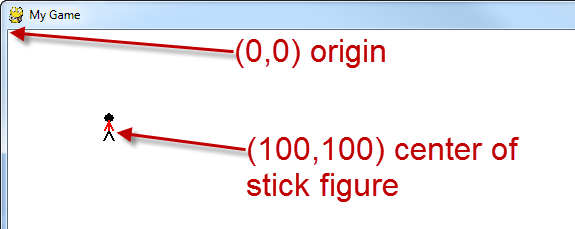
\includegraphics[scale=0.5]{ressources/positionnement.png}
\end{center}
\end{minipage}

Une image \textbf{bitmap} est généralement stockée dans un format de \textbf{fichier binaire}, comme PNG, JPEG \ldots Ces fichiers ne sont pas lisibles par l'homme, ce sont des suites d'\textbf{octets}. Le nombre d'octets codant un pixel définit la \textbf{profondeur} de l'image : par exemple  1 octet soit 8 bits pour une image en niveaux de gris ou 3 octets soit 24 bits pour une image en couleurs. Pour éditer un fichier binaire, il faut un éditeur hexadécimal comme l'éditeur en ligne \url{https://hexed.it/}.

Une image \textbf{bitmap}, peut aussi être stockée, dans un format de \textbf{fichier texte}, comme PBM, PGM, PPM. Un fichier texte est une suite de caractères lisibles par l'homme, à travers un éditeur de textes comme BlocNote ou NotePad++.

\end{definition}



\begin{exerciceB}{Méta-données d'une image}

Avec l'outil \href{https://www.sno.phy.queensu.ca/~phil/exiftool/}{exiftool}, éditer les méta-données au format \textbf{exif} de l'image \textit{image.jpg} fournie.

\begin{enumerate}
	\item Déterminer le format de fichier, la définition de l'image et sa profondeur en bits.
	\item Déterminer le type d'appareil et le zoom avec lesquels la photographie a été prise.
	\item Déterminer la date et l'heure de la prise de vue ainsi que ses coordonnées géographiques. En déduire la commune et le département où cette photo a été prise.
	
\end{enumerate}

\end{exerciceB}


\newpage

\section{Fichiers textes et images bitmap}


\begin{blocnote}{Lecture / écriture de fichiers textes}

En Python, l'accès à un fichier texte se fait par l'intermédiaire d'un descripteur de fichier créé à l'aide de  \texttt{f = open(nom,mode)}. Une fois que les manipulations sont terminées, il faut bien penser à fermer le descripteur de  fichier avec  \texttt{f.close()}. 


Lors de l'ouverture d'un fichier on précise l'un des trois modes d'accès :  lecture \texttt{'r'},  écriture \texttt{'w'} ou ajout \texttt{'a'}.  Attention, pour l'ouverture en mode écriture, les modes \texttt{'w'} ou \texttt{'a'} créent le fichier s'il n'existe pas mais le mode \texttt{'w'} écrase le fichier s'il existe déjà. 
 
\danger{} Avant de manipuler un fichier texte, il faut  conna\^itre sa structure !!!

\danger{} Un fichier texte se lit comme une bande magnétique, un curseur se déplace dans le fichier de caractère en caractère ou de ligne en ligne.
On ne peut pas accéder à la ligne 100 sans lire  les 99 précédentes !!!



\begin{center}
\begin{longtable}{|l|l|}
\hline  Fonctions & R\^ole \\
\hline
\texttt{f = open('nom\_fichier.txt','w')} & accès en écriture avec création d'un nouveau  fichier \\
\hline
\texttt{f = open('nom\_fichier.txt','r')} & accès à  un fichier existant en mode lecture \\
\hline
\texttt{f = open('nom\_fichier.txt','a')} & accès en écriture à  un fichier existant en mode ajout \\
\hline
\texttt{f.write('texte')} & ajout de 'texte' dans le fichier  \\
\hline
\texttt{f.writelines(liste)} & ajout d'une liste de lignes  dans un fichier  \\
\hline
\texttt{f.read()} & lecture de tout le fichier  \\
\hline
\texttt{f.read(8)} & lecture des 8 premiers caractères du fichier  \\
\hline
\texttt{f.readline()} & lecture de la ligne courante du fichier  \\
\hline
\texttt{f.readlines()} & liste de toutes les lignes à partir de la position courante  \\
\hline
\texttt{f.tell()} & position courante du curseur \\
\hline
\texttt{f.seek(16)} & place le curseur sur le caractère en position 16  \\
\hline
\texttt{for ligne in f} & itération sur les lignes du fichier \\
\hline
\texttt{f.close()} & fermeture du fichier \\
\hline
\end{longtable}
\end{center}


\end{blocnote}


\begin{center}
\begin{longtable}{p{0.45\linewidth}p{0.45\linewidth}}
\begin{center}
\fbox{\textbf{Lecture de tout le fichier}}
\begin{lstlisting}
f = open('fichier.txt','r')
data = f.read()
f.close()
\end{lstlisting}
\end{center}
&
\begin{center}
\fbox{\textbf{Lecture ligne par ligne }}
\begin{lstlisting}
f = open('fichier.txt','r')
for ligne in f:
	#traitement sur la ligne
f.close()
\end{lstlisting}
\end{center} 
\\
 \begin{center}
\fbox{\textbf{Lecture ligne par ligne }}
\begin{lstlisting}
f = open('fichier.txt','r')
ligne = f.readline()
while ligne != '':
	#traitement sur la ligne
	ligne = f.readline()	
f.close()
\end{lstlisting}
\end{center}  

&
\begin{center}
\fbox{\textbf{Capture dans une liste de toutes les lignes}}
\begin{lstlisting}
f = open('fichier.txt','r')
listlignes = f.readlines()
f.close()
\end{lstlisting}
\end{center}
\\
\begin{center}
\fbox{\textbf{Écriture }}
\begin{lstlisting}
f = open('fichier.txt','w')
f.write('Une ligne qui ecrase tout\n')
f.close()
\end{lstlisting}
\end{center}
&
\begin{center}
\fbox{\textbf{Ajout à la fin}}
\begin{lstlisting}
f = open('fichier.txt','a')
f.write('Ligne de plus\n')
f.close()
\end{lstlisting}
\end{center}
\end{longtable}
\end{center}



\begin{exerciceB}{Images binaires au format PBM}

Le format PBM est un format de fichier texte permettant de stocker des images bitmap en noir et blanc. La première ligne du fichier précise le format avec l'identifiant P1, la seconde définit la largeur L et  la hauteur H de l'image et à partir de la troisième ligne le tableau de pixels est stocké ligne par ligne, chaque pixel étant codé par 0 pour un pixel blanc et 1 pour un noir.

On donne ci-dessous l'exemple d'une image de définition $4 \times 5$ représentant un F.

\begin{minipage}{0.45\linewidth}
\begin{center}
\begin{minipage}{0.45\linewidth}
{\Large
\begin{verbatim}
P1
4 5
1 1 1 1
1 0 0 0
1 1 1 0
1 0 0 0
1 0 0 0
\end{verbatim}
}
\end{minipage}
\end{center}
\end{minipage}\hfill
\begin{minipage}{0.45\linewidth}
\begin{center}

\includegraphics[scale=0.5]{ressources/f.png}
\end{center}
\end{minipage}

\begin{enumerate}
	
	\item Déterminer la colonne et la ligne du pixel blanc situé à droite de la barre centrale du F. On commence la numérotation des lignes et des colonnes à partir de 0.
	
	\item Le code ci-dessous permet de créer l'image d'un damier de définition $500 \times 500$ dont les cases sont des carrés de $50$ pixels. La suite de  caractères \lstinline+'\n'+ code un caractère spécial, le  \textbf{saut de ligne}.

\bigskip

\begin{minipage}{0.8\linewidth}
\begin{lstlisting}
L, H = 500, 500
f = open('damier.pbm', 'w')
f.write('P1\n')
f.write(str(L) + ' ' + str(H) + '\n')
for lig in range(H):
	for col in range(L):
    	f.write(str((lig // 50 + col // 50) % 2) + ' ')
    f.write('\n')
f.close()
\end{lstlisting}
\end{minipage}\hfill
\begin{minipage}{0.2\linewidth}

\includegraphics[scale=0.23]{ressources/damier.png}
\end{minipage}



Écrire un code qui génère l'image ci-dessous, de définition $500 \times 500$, constituée de bandes noires parallèles dont les côtés coincidant avec un  bord de l'image, mesurent $50$ pixels.

\begin{center}
\fbox{\textbf{Image à générer}}

\bigskip


\includegraphics[scale=0.25]{ressources/bandes.png}
\end{center}

\item Recopier et compléter la fonction \lstinline+inverser_couleurs_pbm(source, but)+ qui crée un fichier de format PBM \texttt{but} obtenu à partir d'un fichier PBM \texttt{source} en inversant les valeurs de chaque pixel ( 0 devient 1 et vice-versa).

\begin{lstlisting}
def inverser_couleurs_pbm(source, but):
    """Lit le fichier pbm  source  et le recopie dans le fichier pgm
    but en inversant les couleurs"""
    #ouverture de fichiers en  lecture pour source et écriture pour but
    f = open(source, 'r')
    g = open(but, 'w')
    #on recopie l'en-tête (les deux premières lignes)
    for k in range(2):
        lig = f.readline()
        g.write(lig)
    #pour les lignes codant les pixels on inverse chaque valeur de pixel
    for lig in f:
        for caractere in lig:
            #à compléter
    g.close()
    f.close()
\end{lstlisting}



\end{enumerate}

\end{exerciceB}

%\newpage

\begin{exerciceB}{Images en niveaux de gris au format PGM}

Le format PGM est un format de fichier texte permettant de stocker des images en niveaux de gris. La première ligne du fichier précise le format avec l'identifiant P2, la seconde définit la largeur L et  la hauteur H de l'image et  la troisième fixe la valeur maximale de niveau de gris.

À partir de la quatrième ligne le tableau de pixels est stocké ligne par ligne, chaque pixel est  codé par son niveaux de gris  entre le minimum 0 et le maximum (255 en général). 

On donne ci-dessous l'exemple de l'image \texttt{lena.ppm} fournie avec les ressources du DM. Seuls les six premiers pixels des deux premières lignes du tableau de pixels sont représentés.

\begin{minipage}{0.45\linewidth}
\begin{center}
\begin{minipage}{0.45\linewidth}
{\Large
\begin{verbatim}
P2
512 512
255
162 162 164 162 161 157 ....
162 162 164 162 161 157 ....
\end{verbatim}
}
\end{minipage}
\end{center}
\end{minipage}\hfill
\begin{minipage}{0.4\linewidth}
\begin{center}
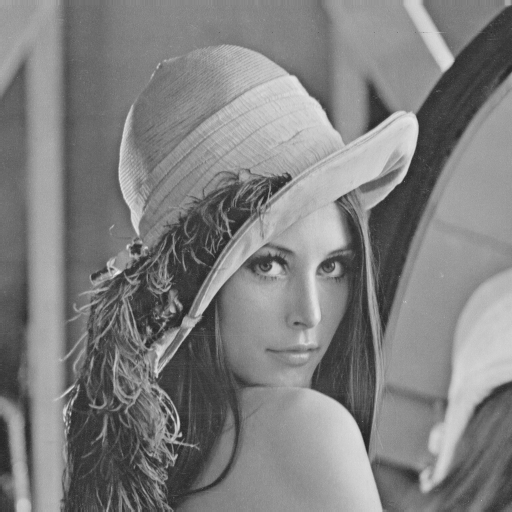
\includegraphics[scale=0.3]{ressources/lenagray.png}
\end{center}
\end{minipage}

\begin{enumerate}
	
	\item Dans une image au format PGM, le niveau de gris d'un pixel est  codé  sur un nombre variable de caractères de 1 à 3, alors que dans un format binaire comme PNG, le niveau de gris est stocké sur un seul octet. Un fichier texte est donc plus lisible par un humain mais un fichier binaire est plus compact et plus facile à manipuler par la machine.

Pour découper en pixels  une ligne du tableau de pixels dans un fichier PGM, il faut utiliser la méthode \texttt{split} des chaînes de caractères.

\begin{lstlisting}
In [19]: ligne = "162 162 164 162 161 157"

In [20]: liste_pixels = ligne.split()

In [21]: liste_pixels
Out[21]: ['162', '162', '164', '162', '161', '157']
\end{lstlisting}

À l'aide des indications précédentes, écrire une fonction une fonction \lstinline+rechercher_pixel_ppm(source, lig, col)+ qui retourne la valeur entière du pixel situé en ligne \texttt{lig} et colonne \texttt{col} dans un fichier image \texttt{source} au format PGM. Attention, il faut penser à sauter les trois lignes d'en-tête du fichier !

\begin{lstlisting}
In [22]: rechercher_pixel_ppm("lena.ppm", 1, 5)
Out[22]: 157
\end{lstlisting}

\item On a expliqué précédemment comment découper la ligne d'un fichier PGM en liste de pixels. Le \texttt{slicing}  et la méthode \texttt{join} des listes permettent d'inverser la liste et de reconstruire une ligne correspondante en séparant chaque pixel par un espace.

\begin{lstlisting}
In [25]: liste_pixels
Out[25]: ['162', '162', '164', '162', '161', '157']

In [26]: liste_pixels[::-1]
Out[26]: ['157', '161', '162', '164', '162', '162']

In [27]: ' '.join(liste_pixels[::-1])
Out[27]: '157 161 162 164 162 162'
\end{lstlisting}

Écrire une fonction \lstinline+flip_ppm(source, but)+ qui ouvre un fichier image \texttt{source} au format PGM et le recopie dans un  un fichier image \texttt{but} au format PGM en appliquant à l'image un flip \ie{} une symétrie axiale par rapport au bord droit de l'image.

Tester la fonction sur l'image \texttt{lena.ppm}.

\begin{tabular}{*{3}{c}}
\begin{minipage}{0.4\linewidth}
\begin{center}
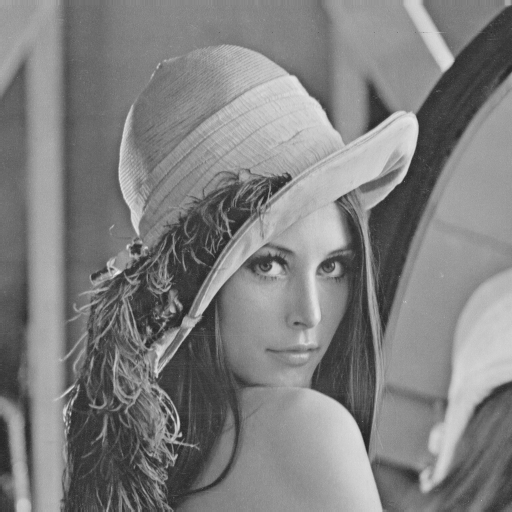
\includegraphics[scale=0.3]{ressources/lenagray.png}
\end{center}
\end{minipage}
&
$\overset{\text{\textbf{Flip}}}{\Longrightarrow}$
&
\begin{minipage}{0.4\linewidth}
\begin{center}
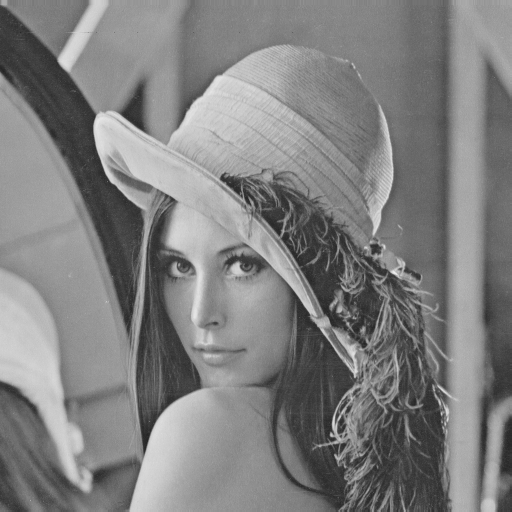
\includegraphics[scale=0.3]{ressources/lena-flip.png}
\end{center}
\end{minipage}
\end{tabular}


\item Dans un fichier texte, on ne peut accéder à la dernière ligne qu'en parcourant d'abord toutes les précédentes. La méthode \texttt{readlines} permet de  stocker dans une liste toutes les lignes d'un fichier texte  à partir de la position courante et l'itérateur \texttt{reversed} permet de parcourir une liste dans l'ordre inverse.

Le code ci-dessous permet de recopier le fichier \texttt{endroit.txt} dans le fichier \texttt{envers.txt} en gardant la première ligne mais en inversant l'ordre des lignes suivantes.

\begin{minipage}{0.6\linewidth}

\begin{center}
\fbox{Code}

\bigskip


\begin{lstlisting}
f = open('endroit.txt', 'r')
g = open('envers.txt', 'w')
#saut de la première ligne
lig = f.readline() 
g.write(lig)
liste_lignes = f.readlines()
for lig in reversed(liste_lignes):
    g.write(lig)
f.close()
g.close()
\end{lstlisting}
\end{center}
\end{minipage}\hfill
\begin{minipage}{0.15\linewidth}

\begin{center}
\fbox{\texttt{endroit.txt}}

\bigskip

\begin{verbatim}
#En-tete
0 0 0
1 1 1
2 2 2
\end{verbatim}
\end{center}
\end{minipage}\hfill
\begin{minipage}{0.15\linewidth}


\begin{center}
\fbox{\texttt{envers.txt}}

\bigskip

\begin{verbatim}
#En-tete
2 2 2
1 1 1
0 0 0
\end{verbatim}
\end{center}
 
\end{minipage}


À l'aide des indications précédentes, écrire une fonction \lstinline+flop_ppm(source, but)+  qui ouvre un fichier image \texttt{source} au format PGM et le recopie dans un  un fichier image \texttt{but} au format PGM en appliquant à l'image un flop \ie{} une symétrie axiale par rapport au bord supérieur de l'image.

Tester la fonction sur l'image \texttt{lena.ppm}.

\begin{tabular}{*{3}{c}}
\begin{minipage}{0.4\linewidth}
\begin{center}
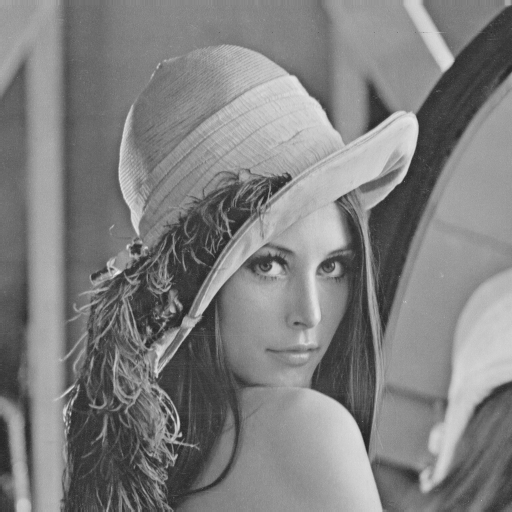
\includegraphics[scale=0.3]{ressources/lenagray.png}
\end{center}
\end{minipage}
&
$\overset{\text{\textbf{Flop}}}{\Longrightarrow}$
&
\begin{minipage}{0.4\linewidth}
\begin{center}
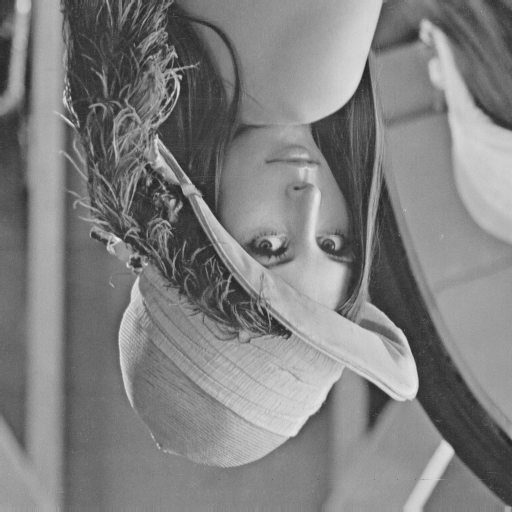
\includegraphics[scale=0.3]{ressources/lena-flop.png}
\end{center}
\end{minipage}
\end{tabular}
\end{enumerate}

\end{exerciceB}

\section{Fichiers binaires et images bitmap}




Le fichier \texttt{lenagray.png} fourni avec les ressources du DM, stocke la même image que \texttt{lena.ppm} mais comme un fichier binaire au format PNG, \ie{} comme une suite  d'octets qui n'est pas lisible par l'homme. Après un en-tête spécifique au format et précisant les dimensions de l'image, le niveau de gris de chaque pixel est codé sur un octet (trois si l'image était en couleur, voir plus si on code aussi la transparence). 

Si on édite le fichier avec un éditeur hexadécimal comme Okteta ou l'éditeur en ligne \url{https://hexed.it/}, on obtient à gauche les octets codés sur deux chiffres en hexadécimal (base 16) et à droite leurs traductions en caractères dans un  jeu de caractères ASCII (ici le jeu étendu ISO-8859-1). Par exemple, le niveau de gris $75=4 \times 16 + 11$ correspondra à l'octet \texttt{4b} en hexadécimal et au caractère \texttt{K}.

\begin{center}
	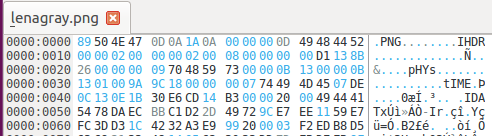
\includegraphics[scale=0.7]{ressources/fichier-binaire.png}
\end{center}

On peut déchiffrer à partir du deuxième octet du fichier l'identifiant PNG du format. Ainsi le caractère \texttt{P}, qui  a pour ordinal $80$ dans le jeu de caractères, correspond à l'octet $50$ en hexadécimal puisque $80 = 5 \times 16 + 0$.

\begin{lstlisting}
In [17]: int('0x50', 16)     #conversion en base dix de 50 en base seize                                                   
Out[17]: 80

In [18]: chr(80)            #caractère unicode d'ordinal 80                                              
Out[18]: 'P'
\end{lstlisting}


\begin{exerciceB}{Transformation du photomaton}

On considère une image bitmap de dimensions $n \times n$ avec $n$ pair, comme \texttt{lenagray.png} de dimensions $512 \times 512$.

Les lignes sont indexées de $j = 0$ à $j = n-1$ et les colonnes de $i = 0$ à $i = n - 1$.

À partir du tableau de pixels de cette image \texttt{source}, on construit le tableau de pixels d'une image \texttt{but} selon la transformation suivante appelée \textbf{transformation du photomaton}.

\begin{center}
\begin{tabular}{lcr}

\begin{minipage}{0.4\linewidth}
\begin{center}

\begin{tikzpicture}[scale=0.85]

\draw (0,0) grid (8,8);
\draw (0.5, 7.5) node {A};
\draw (1.5, 7.5) node {B};
\draw (0.5, 6.5) node {C};
\draw (1.5, 6.5) node {D};
\draw (2.5, 7.5) node {a};
\draw (3.5, 7.5) node {b};
\draw (2.5, 6.5) node {c};
\draw (3.5, 6.5) node {d};
\draw (0.5, 8) node[above] {$i=0$};
\draw (1.5, 8) node[above] {$i=1$};
\draw (0, 7.5) node[left] {$j=0$};
\draw (0, 6.5) node[left] {$j=1$};

\end{tikzpicture}


\end{center}
\end{minipage}

&

 $\overset{\text{\textbf{Photomaton}}}{\Longrightarrow}$


&


\begin{minipage}{0.4\linewidth}
\begin{center}

\begin{tikzpicture}[scale=0.85]

\draw (0,0) grid (8,8);
\draw (0.5, 7.5) node {A};
\draw (4.5, 7.5) node {B};
\draw (0.5, 3.5) node {C};
\draw (4.5, 3.5) node {D};
\draw (1.5, 7.5) node {a};
\draw (5.5, 7.5) node {b};
\draw (1.5, 3.5) node {c};
\draw (5.5, 3.5) node {d};
\draw (0.5, 8) node[above] {$i=0$};
\draw (1.5, 8) node[above] {$i=1$};
\draw (0, 7.5) node[left] {$j=0$};
\draw (0, 6.5) node[left] {$j=1$};
\draw[very thick] (4,0) -- (4,8);
\draw[very thick] (0,4) -- (8,4);
\end{tikzpicture}


\end{center}
\end{minipage}




\end{tabular}


\end{center}


\begin{itemize}

	\item On découpe l'image en petits carrés de dimensions $2 \times 2$ et l'image en quatre secteurs carrés de dimensions $\frac{n}{2} \times \frac{n}{2}$.
	
	\item Pour chaque petit carré :
	
	\begin{itemize}
		
		\item Le pixel en haut à gauche de coordonnées $(i, j)$ avec $i$ pair et $j$ pair est envoyé dans le secteur en haut à gauche de l'image, en position $\left(i//2, \, j//2\right)$.
	
	\item \textcolor{red}{Le pixel en haut à droite de coordonnées $(i, j)$ avec $i$ impair et $j$ pair est envoyé dans le secteur en haut à droite de l'image, en position $\left((i+n)//2, \, j//2\right)$.}
	
	\item \textcolor{red}{Le pixel en bas à gauche de coordonnées $(i, j)$ avec $i$ pair et $j$ impair est envoyé dans le secteur en bas à gauche de l'image, en position $\left(i//2, \, (n + j) //2\right)$.}

	\item Le pixel en bas à droite de coordonnées $(i, j)$ avec $i$ impair et $j$ impair est envoyé dans le secteur en bas à droite de l'image, en position $\left((i+n)//2, \, (j+n)//2\right)$.
	
\end{itemize}

\item Ainsi, on construit une correspondance unique entre un pixel de l'image \texttt{source} et un pixel de l'image \texttt{but}. La transformation du photomaton est une  \textbf{transformation bijective} du tableau de pixels.

\item Voici un exemple d'application de la transformation du photomaton à un tableau de pixels de dimensions $4 \times 4$ :


\begin{tabular}{*{3}{c}}
\begin{minipage}{0.42\linewidth}
\begin{center}
\begin{tabular}{*{4}{c}}
1 & 2& 3& 4 \\
5 & 6 & 7 & 8 \\
9 & 10 & 11 & 12 \\
13 & 14 & 15 & 16
\end{tabular}
\end{center}
\end{minipage}
&
$\overset{\text{\textbf{Photomaton}}}{\Longrightarrow}$
&
\begin{minipage}{0.42\linewidth}
\begin{center}
\begin{tabular}{*{4}{c}}
1 & 3 & 2& 4 \\
9 & 11 & 10 & 12 \\
5 & 7 & 6 & 8 \\
13 & 15 & 14 & 16
\end{tabular}
\end{center}
\end{minipage}
\end{tabular}

\end{itemize}

 
Si on applique par itérations successives la transformation du photomaton à partir de  \texttt{lennagray.png},  image source de dimensions $512 \times 512$, voici les images itérées qu'on obtient :

\bigskip

\begin{tabular}{*{3}{c}}

\begin{minipage}{0.3\linewidth}
\begin{center}
\fbox{Source}

\bigskip


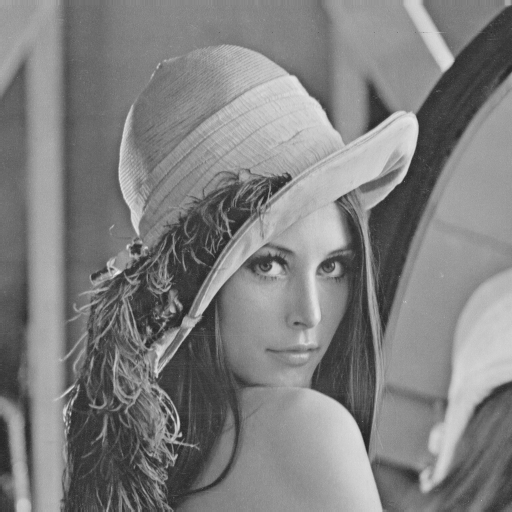
\includegraphics[scale=0.25]{ressources/lenagray.png}
\end{center}

\end{minipage}

&

\begin{minipage}{0.3\linewidth}
\begin{center}
\fbox{Itération 1}

\bigskip

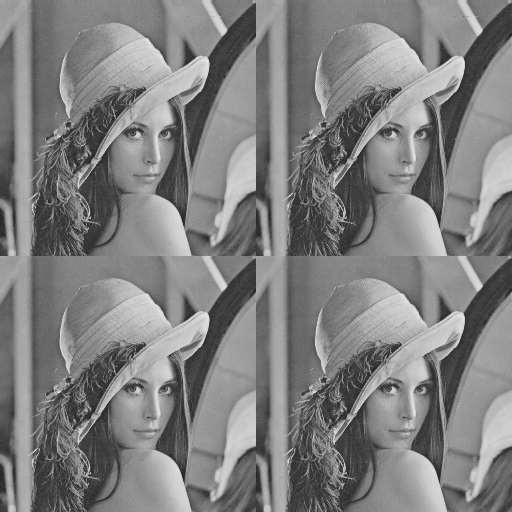
\includegraphics[scale=0.25]{ressources/lenagray-photomaton-iteration-1.png}
\end{center}
\end{minipage}

&

\begin{minipage}{0.3\linewidth}
\begin{center}
\fbox{Itération 2}

\bigskip

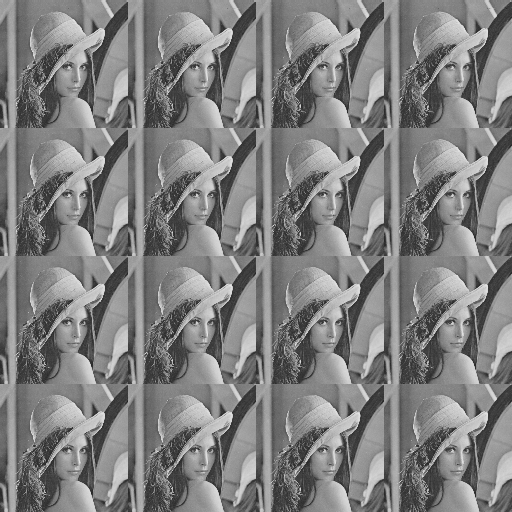
\includegraphics[scale=0.25]{ressources/lenagray-photomaton-iteration-2.png}
\end{center}
\end{minipage}

\\

&

&



\\
\begin{minipage}{0.3\linewidth}
\begin{center}
\fbox{Itération 3}

\bigskip

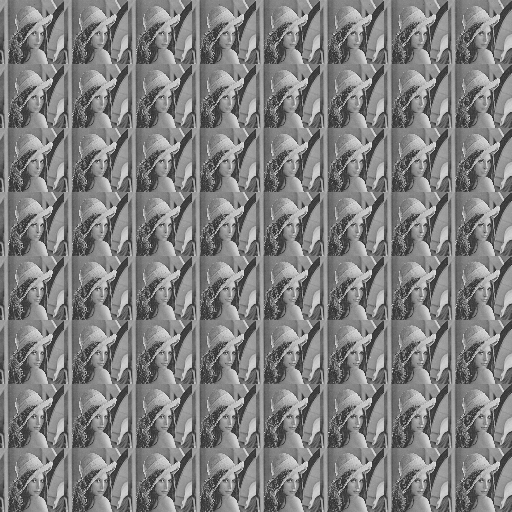
\includegraphics[scale=0.25]{ressources/lenagray-photomaton-iteration-3.png}
\end{center}

\end{minipage}



&
\begin{minipage}{0.3\linewidth}
\begin{center}
\fbox{Itération 4}

\bigskip

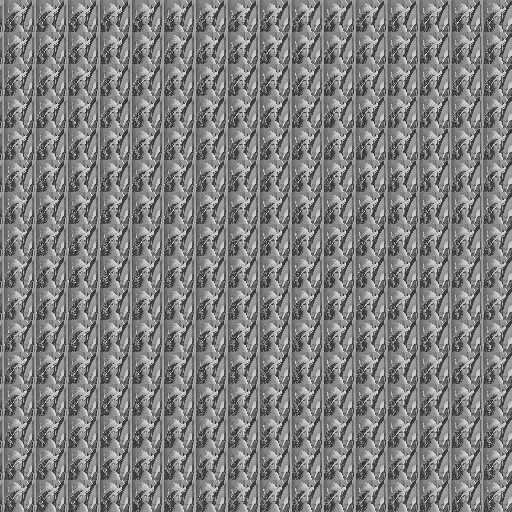
\includegraphics[scale=0.25]{ressources/lenagray-photomaton-iteration-4.png}
\end{center}
\end{minipage}

&

\begin{minipage}{0.3\linewidth}
\begin{center}
\fbox{Itération 5}

\bigskip


\includegraphics[scale=0.25]{ressources/lenagray-photomaton-iteration-5.png}
\end{center}
\end{minipage}

\end{tabular}

\begin{blocnote}{Modules \texttt{PIL} et  \texttt{numpy}}

\begin{itemize}[label=\ding{43}]
	
	\item Nous allons naturellement représenter le tableau de pixels d'une image bitmap par  une liste de listes ou tableau à deux dimensions (matrice en mathématiques). Pour ouvrir les fichier images, on  va utiliser \texttt{Image} le sous-module du module \texttt{PIL}, qui va nous renvoyer des objets spécifiques qui ne se convertissent pas en listes de listes mais en \texttt{ndarray} avec le module \texttt{numpy}. Nous manipulerons ces derniers comme des listes de listes. 
	
	\item Les modules \texttt{numpy} et \texttt{PIL} (en fait son fork \texttt{pillow}) sont inclus dans la distribution \texttt{Anaconda} mais si on a juste installé la distribution standard de \texttt{Python}, on peut les installer depuis un interpréteur de commandes du système (\texttt{cmd.exe} sous Windows) avec les commandes  :  

\begin{lstlisting}
C:\python3 -m pip install numpy
C:\python3 -m pip install pillow
\end{lstlisting}

\item Pour extraire le tableau de pixels d'une image bitmap stockée dans un fichier binaire comme \texttt{lengray.png}, on utilise \lstinline+Image.open+ du module \texttt{PIL}  puis \lstinline+np.asarray+ du module \texttt{numpy}.

\danger{} Attention, pour que Python trouve le fichier image, il est recommandé de  placer ce fichier dans le même dossier que le script et de  régler le répertoire de travail avec par  exemple l'option \og{} Exécuter le fichier en tant que script  \fg{} sous \texttt{Pyzo}. 



\begin{lstlisting}
In [5]: from PIL import Image

In [6]: import numpy

In [7]: im = Image.open('lenagray.png')

In [8]: tab = numpy.asarray(im)

In [9]: tab
Out[9]: 
array([[162, 162, 164, ..., 166, 153, 129],
       [162, 162, 164, ..., 166, 153, 129],
       [162, 162, 164, ..., 166, 153, 129],
       ..., 
       [ 54,  54,  59, ..., 110, 105, 106],
       [ 53,  53,  63, ..., 109, 111, 113],
       [ 53,  53,  63, ..., 109, 111, 113]], dtype=uint8)

In [10]: tab[1][2]   #pixel en deuxième ligne et troisième colonne
Out[10]: 164
\end{lstlisting}

\item \danger{} Attention, comme on le voit ci-dessus le pixel de coordonnées (colonne, ligne) = (2, 1)  est accessible par \lstinline+tab[1][2]+. On indexe d'abord la ligne (l'ordonnée)  puis la colonne (l'abscisse) et on rappelle que les deux sont numérotées à partir de $0$.

\item Réciproquement, une fois le traitement sur le  tableau de pixels effectué, on peut construire l'image associée. Dans un premier temps, on  convertit le tableau en \texttt{ndarray} pour  l'interface avec \texttt{Image} puis on utilise \texttt{Image.fromarray} pour construire une image  qu'on enregistre l'image sur le disque avec la méthode \texttt{save}.

\danger{} Pour que le tableau de pixels corresponde bien à une image en niveau de gris, il faut préciser le type \texttt{'uint8'} lors de la conversion en \texttt{ndarray}.

\begin{lstlisting}
In [12]: tab = [ [0 for col in range(512)] for lig in range(512)]

In [13]: type(tab)
Out[13]: list

In [14]: tab = numpy.array(tab, dtype = 'uint8')  #liste -> ndarray

In [15]: type(tab)    
Out[15]: numpy.ndarray

In [16]: im = Image.fromarray(tab)

In [17]: im.save('tableau-noir.png')   #sauver l'image sur le disque

In [18]: im.show()       #afficher l'image avec la visionneuse
\end{lstlisting}

\end{itemize}


\end{blocnote}

\begin{enumerate}

	\item Écrire une fonction \lstinline+transformation(i, j, n)+ qui retourne les coordonnées de l'image du pixel de coordonnées \texttt{(i, j)} par la transformation du photomaton.
	
	\item On donne ci-dessous le code d'une fonction \lstinline+copie(tableau)+ qui retourne la copie profonde d'un tableau de pixels (liste de listes) sous forme de \texttt{ndarray}.
	
\begin{lstlisting}
def copie(tableau):
    """Retourne la copie profonde d'un tableau à deux dimensions"""
    return numpy.array([[tableau[j][i] for i in range(len(tableau[j]))] 
    for j in range(len(tableau))], dtype = 'uint8')
\end{lstlisting}

À l'aide de cette fonction, écrire une fonction \lstinline+photomaton(tableau)+ qui retourne le tableau calculé après application de la fonction photomaton au tableau de pixels passé en paramètre.

\item Recopier et compléter le code de la  fonction \lstinline+ photomaton_iterer(source, k)+ qui itère \texttt{k} fois la fonction photomaton à partir du fichier image \texttt{source} et enregistre à chaque itération  au format \texttt{png}, l'image correspondant au tableau de pixels obtenu.


\begin{lstlisting}
def photomaton_iterer(source, k):
    im = Image.open(source)
    nom, extension = source.split('.')
    tab = numpy.asarray(im)
    for iteration in range(1, k + 1):
   		#to be completed
\end{lstlisting}


\item Que remarque-t-on si on itère $9$ fois la fonction photomaton à partir de l'image  \texttt{lenagray.png}, de dimensions $512 \times 512$ ?

\item Tester la fonction \lstinline+ photomaton_iterer(source, k)+ sur des images sources de dimensions $128 \times 128$ ou $256 \times 256$ en essayant de retrouver le même phénomène que pour une image de dimensions $512 \times 512$.

Quelle conjecture peut-on faire ?

	
\end{enumerate}


\end{exerciceB}



 \end{document}
